% REMEMBER: You must not plagiarise anything in your report. Be extremely careful.

\documentclass{l4proj}

    
%
% put any additional packages here
\usepackage{multirow}
%

\begin{document}

%==============================================================================
%% METADATA
\title{Creating a server for protein disorder prediction based on deep neural networks}
\author{Ryan Gregson}
\date{March, 2023}

\maketitle

%==============================================================================
%% ABSTRACT
\begin{abstract}
    Every abstract follows a similar pattern. Motivate; set aims; describe work; explain results.
    \vskip 0.5em
    ``XYZ is bad. This project investigated ABC to determine if it was better. 
    ABC used XXX and YYY to implement ZZZ. This is particularly interesting as XXX and YYY have
    never been used together. It was found that  
    ABC was 20\% better than XYZ, though it caused rabies in half of subjects.''
\end{abstract}

%==============================================================================

% EDUCATION REUSE CONSENT FORM
% If you consent to your project being shown to future students for educational purposes
% then insert your name and the date below to  sign the education use form that appears in the front of the document. 
% You must explicitly give consent if you wish to do so.
% If you sign, your project may be included in the Hall of Fame if it scores particularly highly.
%
% Please note that you are under no obligation to sign 
% this declaration, but doing so would help future students.
%
\def\consentname {Ryan Gregson} % your full name
\def\consentdate {1 March 2023} % the date you agree
%
\educationalconsent


%==============================================================================
\tableofcontents

%==============================================================================
%% Notes on formatting
%==============================================================================
% The first page, abstract and table of contents are numbered using Roman numerals and are not
% included in the page count. 
%
% From now on pages are numbered
% using Arabic numerals. Therefore, immediately after the first call to \chapter we need the call
% \pagenumbering{arabic} and this should be called once only in the document. 
%
% Do not alter the bibliography style.
%
% The first Chapter should then be on page 1. You are allowed 40 pages for a 40 credit project and 30 pages for a 
% 20 credit report. This includes everything numbered in Arabic numerals (excluding front matter) up
% to but excluding the appendices and bibliography.
%
% You must not alter text size (it is currently 10pt) or alter margins or spacing.
%
%
%==================================================================================================================================
%
% IMPORTANT
% The chapter headings here are **suggestions**. You don't have to follow this model if
% it doesn't fit your project. Every project should have an introduction and conclusion,
% however. 
%
%==================================================================================================================================
\chapter{Introduction}

% reset page numbering. Don't remove this!
\pagenumbering{arabic} 

\section{Motivation}

Intrinsically disordered proteins do not have a fixed or ordered three-dimensional structure and there are significant differences between the amino acid sequences of intrinsically disordered proteins (IDPs) / intrinsically disordered regions (IDRs) compared to structured globular (functional) proteins \citep{Martinelli:19}. Figure \ref{fig:structured prot} demonstrates the difference between unstructured and structured proteins, where a solid ribbon-like representation is used to depict the well-defined three-dimensional structure, such as alpha helices and beta sheets, and disordered regions of the proteins are depicted using thinner strands, indicating the lack of fixed structure. The structural order of these sequences can be manually labelled from experiments with x-ray crystallographic analysis \citep{idp_wiki}. These experiments can be difficult and the number of newly occurring proteins submitted to the Protein Data Bank (PDB) \citep{pdb} each year makes it difficult to manually experiment with each one, meaning many proteins’ disorder structure have not been assessed.

\begin{figure}[!htb]
    \centering
    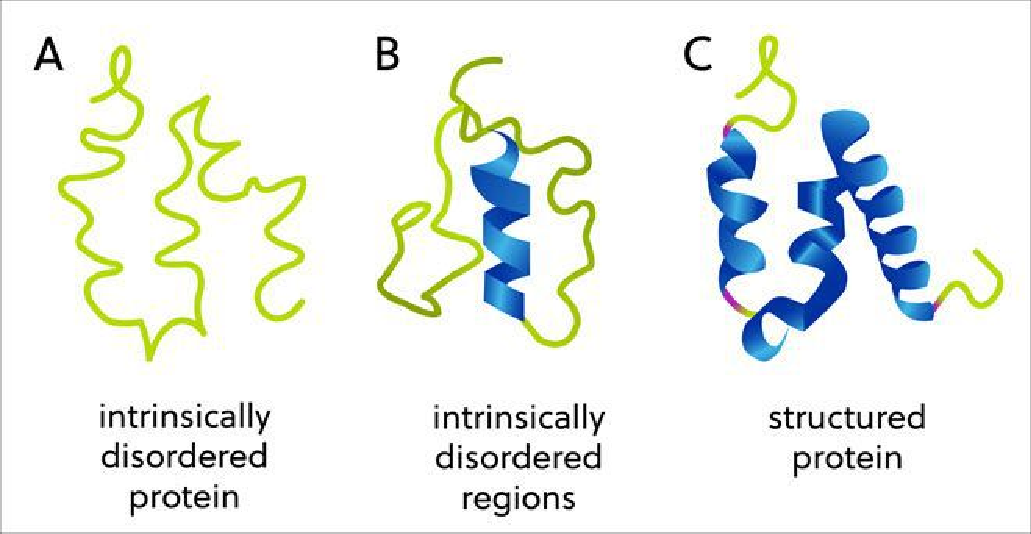
\includegraphics[width=\linewidth]{images/structprot.pdf}

    \caption{An example of ordered and disordered proteins \citep{Tenchov:22}. Proteins that are disordered do not have a defined or fixed structure, in contrast to ordered proteins.}
    \label{fig:structured prot} 
\end{figure}

We can use bioinformatic tools to label the disordered regions in these protein sequences by creating a model that can learn the differences between ordered and disordered amino acid sequences. With more labelled sequences, doctors and researchers can understand more about disordered protein sequences. Insights about these disordred regions helps drive research for the development of drugs that are applied to disordered proteins, understanding the functionality of these regions and contributes to keeping a well-maintained knowledge database of proteins. It is important this research is supported as disordered proteins cause neurodegenerative diseases such as Alzheimer’s, Parkinson’s and Huntington’s. Therefore, it is important drugs can be designed and applied to IDPs in an attempt to counteract these diseases. Furthermore, some disordered regions in proteins are vital for creating functionality in the protein as they can give elastic properties to proteins. These elastic properties are usually difficult to create with ordered protein chains. An example of this is the entropic spring in Titin, which is composed of both ordered and disordered regions \citep{Morgan:17}. This entropic spring allows muscle fibres to stretch and contract efficiently, making it an essential component of muscle function and demonstrating that IDPs can be useful within our bodies.

Deep learning approaches have become incredibly popular recently, and these approaches currently dominate classification tasks. Deep learning architectures are prevalent in classifying the IDRs in protein sequences, where state of the art predictors such as SPOT-DISORDER2 \citep{Hanson:19} also have their own online protein disorder prediction servers for others to use their deep learning model.

\section{General problem and aim}

Protein sequences are made up of amino acids. The problem we are attempting to solve is to see if we can use these sequences to predict whether each amino acid is ordered or disordered, hence identifying the intrinsically disordered regions. We will produce deep neural networks which will take in protein sequences and predict the disordered regions within them. 

The aim of this project is to explore how different deep learning approaches and architectures perform at predicting protein disorder. To assess these deep learning methods, we will: 
\begin{itemize}
    \item Discuss current solutions to protein disorder prediction.
    \item Discuss our approach for creating a protein disorder classifier.
    \item Design and implement different deep neural networks, such as a convolutional neural network (CNN) and recurrent neural network (RNN). 
    \item Evaluate our implemented neural networks using standard metrics and the test datasets proposed by CASP \citep{casp}, which have been used for evaluating protein disorder prediction models. 
\end{itemize}
An aim alongside comparing the deep neural networks is to create a web server, where a user can input a protein sequence via a web page form and see the predictions of disordered regions. This will make my models accessible, which will result in bioscience researchers being able to interact with my developed solution easily.


%==================================================================================================================================
\chapter{Background}
\label{chap:background}

\section{Biology overview}

\subsection{What is a protein?}

Proteins are a linear sequence of amino acids \citep{prot_struct_lib}. The Insulin protein has a precursor molecule with a linear sequence of 110 amino acids (Figure \ref{fig:sequence example}). This globular protein controls blood sugar levels, and diabetics need to inject human insulin to control their blood sugar.

\begin{figure}[!h]
    \centering
    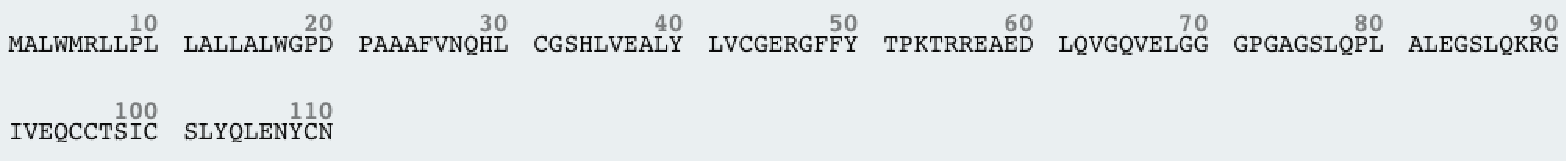
\includegraphics[width=\linewidth]{images/bgseq.pdf}

    \caption{Human insulin amino acid sequence as presented by UniProt. \citep{uniprot:22}. Insulin was the first protein ever sequenced, obtained by Frederick Sanger in 1955.}

    \label{fig:sequence example} 
\end{figure}

There are twenty possible amino acids that protein sequences can be built from, and each of these amino acids have a unique side chain which have different structural properties \citep{aa_wiki}. Different proteins have different sequences of amino acids. The amino acids in the sequence will "interact with each other to form a well-defined, folded protein" \citep{protein_folding}. The folded protein with have a three-dimensional structure, and this three-dimensional structure determines the protein's function \citep{bbc_bitesize}. This function can be supporting frameworks inside cells, catalysing biological reactions, communication between different parts of the body and proteins are used for function inside the immune system \citep{bbc_bitesize}. Therefore, it is important that the folding of proteins is done correctly as misfolded proteins will lose their structure and function, such as the above insulin molecule, which can lead to diseases.

\subsection{Intrinsically disordered proteins (IDPs)}
\label{chap:background sec:IDPs}

IDPs are different to structured proteins. These unstructured, disordered proteins are suggested to cause a number of diseases. For example, disordered mutations of the functional insulin molecule can form amyloid structures. These structures can lead to amyloid disease, such as Alzheimer's, and Parkinson's. IDPs amino acid sequences differ and contain a “low content of bulky hydrophobic amino acids and a high proportion of polar and charged amino acids” \citep{idp_wiki}. In comparison to structured proteins that fold correctly these sequences cannot fold into stable globular proteins, meaning that the protein lacks an ordered three-dimensional structure. The root cause of this lack of structure, causing disorder, is the proteins’ primary structure: the amino acid sequence. When disordered amino acids are grouped, this is labelled as an intrinsically disordered region (IDR) and is where the misfolding occurs. Therefore, making predictions about the probability that an amino acid residue is ordered or disordered within a protein sequence will help determine where this incorrect folding will occur. This means by focusing on the amino acids’ structure we can determine the outcome of the protein functioning correctly. 

A current problem is the lack of labelled data about the structure of protein sequences as determining these via experiments such as nuclear magnetic resonance (NMR) and small-angle X-ray scattering (SAXS) is very costly and time-consuming \citep{disordered_prot_genus_camelus}. To tackle this challenge, bioinformatic tools have been created for protein sequence structure labelling. These tools are often accessible via a web server, such as the DISOPRED server \citep{disopred3_paper}, which uses machine learning methods to make predictions. This project will produce a similar tool for classifying intrinsically disordered proteins after experimentation with different deep learning architectures and approaches.

\section{Deep learning overview}

\subsection{Deep Neural Networks}

Deep neural networks are made up of stacked neural network layers. As these layers are stacked, the output of one layer will be used as input to the next layer in the network. Each of these layers performs feature extraction on their input. Each neural network layer consists of an arbitrary number of neurons with associated weights and bias parameters that are updated throughout training. During training, inputs are classified by the model during a forward pass through the model. These predictions are compared to the true value using a loss function. Through the process of backpropagation \citep{Goodfellow-et-al-2016}, the outcome of the loss function is used and the parameter weights within the network are changed in an aim to improve the models' predictions. To complete this training step, an optimisation method will update each layer of the network, changing the weights of the model as proposed by backpropagation. This training procedure is done with each item in the training set and for multiple iterations of the entire training set, to solve the optimisation problem by minimising the loss and finding optimum weights for the neural network. The machine learning framework, PyTorch \citep{pytorch}, provides the functionality to build neural network layers that extract features; use a loss function with an implemented backpropagation method, and create an optimiser to update a deep neural network model during training. PyTorch also provides efficient tensor computations and can utilise GPUs while training. This software will be useful for creating our deep neural networks due to its efficiency and comprehensive components.

\subsection{Convolutional Neural Networks (CNNs)}

A CNN is a type of neural network that uses convolution kernels to extract features from an input. Convolution kernels can be 1D kernels of size $1\times K$ primarily used for sequence or series data, or 2D kernels of size $N\times M$ primarily used for classifying images. These kernels move across a grid shaped input, checking if a feature is present. With our protein sequences, we can use a kernel of $1\times K$ to slide along a $1\times sequence length$ grid, treating each amino acid as a different input channel and capturing unique features. We can also represent protein sequences as images by creating a $20\times sequence length$ length grid, where each amino acid is a $20\times 1$ vector and this lets us use a different 2D convolution kernel over the protein sequence. These are discussed further in our design (Section \ref{chap:design section:cnn}).

In classification tasks convolution kernels are translation-invariant and require few parameters. These are beneficial as this means it does not matter where the location of the disordered region exists in the sequence. Less parameters means the model can be trained well with smaller training sets. This is good as the labelled datasets from manually curated databases for disordered proteins, such as Disprot \citep{disprot}, are small in comparison to the data provided for other deep learning tasks. \cite{disopred3_paper} have stated further annotated training labels will be beneficial to train protein disorder prediction tools; therefore, using a model architecture that can cope with smaller datasets should be effective. \\

\subsubsection{Fully Convolutional Networks \newline}
\label{chap:background sec:FCN}

During most classification tasks, input of the same shape is passed to the CNN. However, with our protein sequence data the lengths of our sequences range from 19 residues (the protein Conantokin-Pr1 \citep{uniprot:22}) to 34350 residues (the muscle protein Titin \citep{uniprot:22}), so we would need to unnecessarily pad many sequences with lots of redundant blank values. Therefore, we have taken an approach to use a fully convolutional network (FCN). Modern classification networks have been adapted to fully convolutional networks by Shelhamer and Long \citep{fcn_seg}, demonstrating that classification can be done using inputs of arbitrary size. Thus, for these protein sequences of varying length, an FCN will be suitable at handling these inputs. 

\subsection{Recurrent Neural Networks (RNNs)}

A RNN is a type of neural network that is well-suited for processing sequential data. Most sequential data that is processed by RNNs are time series or natural language; however, many RNNs handle biological sequences \citep{Hawkins:05}. RNNs can capture sequential dependencies of an input sequence by using hidden states, which help to make predictions about later elements in the sequence. The hidden states are updated at each item of the sequence; using both the current input and the previous hidden state. This allows a RNN to share knowledge about previous information in the sequence, meaning that the hidden state used to make the prediction about a given element of the input sequence has a greater understanding of the context of the sequence.

With protein sequences, using an RNN is useful because maintaining sequential context stores information about the dependencies between adjacent amino acids in a protein sequence, which is important for predicting whether a given amino acid is likely to be part of a disordered region. Specifically, the hidden state will capture the context of the surrounding amino acids, like capturing information using the width of a convolution kernel, and this provides information about the amino acid at a position of the sequence, which helps make accurate predictions about whether it is ordered or disordered. \\

\subsubsection{Long Short-Term Memory (LSTM) networks \newline}

Traditional RNNs experience the vanishing gradient problem. This happens during backpropagation when the gradients become very small, which results in the RNN being incapable of learning long-term dependencies \citep{Arbel:18}. LSTMs address this problem by preserving gradient information using memory cells and gating mechanisms. This controls the information flow through the network, selectively maintaining some previous sequential context, which enables the network to learn long-term dependencies throughout the entire sequence. This can be effective for protein sequences as there are long-term dependencies and relationships between amino acids throughout the sequence, and this additional contextual information can increase the accuracy of predictions about attributes of the protein, such as where the disordered regions are.

\section{Review of current approaches}
\label{sec:current approaches}

There are currently many approaches to protein disorder prediction, with over 100 different predictors proposed \citep{Zhao:22}. Disorder classifiers implement different methods with the main approaches regarded as: composition-based methods (PONDR VLXT \citep{Romero:01}); hydropath-based methods (DISOPRED \citep{Ward:04}); structural methods (IUPred \citep{Dosztanyi:18}); physiochemical methods (FoldIndex \citep{Prilusky:05}); machine learning methods (DISOPRED3 \citep{disopred3_paper}) and the use of meta-predictors (Metapredict \citep{Emenecker:21}). The Critical Assessment of Structure Prediction (CASP) \citep{casp} motivated solutions for identifying disordered regions in target proteins between 2010-12 using CASP9 and CASP10. Results from the CASP10 assessment \citep{CASP10} show that the top disordered region classifiers consist of machine learning and meta-predictor methods \citep{Zhao:22}. CASP has discontinued the evaluation of IDR prediction, however the Critical Assessment of Intrinsic Protein Disorder community (CAID) \citep{Necci:21}, continued to release withheld testing datasets to assess new prediction tools. These assessments found that deep learning predictors had the best performance at identifying disordered regions accurately \citep{Zhao:22}. This motivates a reason for approaching this task using a deep learning method.

As well as performing well for intrinsic disorder prediction, deep learning methods also dominate in other protein structure prediction tasks such as AlphaFold \citep{Jumper:21}. Improved technology has assisted these neural networks to feasibly increase their depth as well as the increase of digitalised labelled data. Studies have analysed different deep learning architectures for protein disorder prediction and state: “that the architectures of current deep learners are considerably diverse,” and there is no decided optimal architecture yet \citep{Zhao:22}. This motivates us to experiment and compare different deep learning architectures. Furthermore, the top performing models in CAID “utilize deep convolutional and/or recurrent neural networks,” \citep{Hu:21} demonstrating these architectures are important for classifiers tackling this prediction task.

\subsection{Convolutional neural networks}
\label{chap:background sec:litrevCNN}

A model using a convolutional neural network architecture will process the amino acid sequence in a sliding window fashion using a convolution kernel. Older competitive machine learning based methods such as DISOPRED, FoldIndex and IUPred use a sliding window within their algorithm, which justifies the feasibility of a convolution kernel. There are not many prominent models which solely use convolutional layers for protein disorder classification. However, two studies propose using a CNN for similar tasks: predicting DNA-protein binding \citep{Zeng:16}, and protein secondary structure prediction \citep{Ema:22}. The first study concludes that experimentation of different CNN architecture design demonstrated improvements to a state-of-the-art solution and this work “will be important for sequence-based tasks in genomics,” \citep{Zeng:16}. This suggests experimentation using a CNN will be useful for classification of disordered regions as we will be using a sequence-based approach with our protein sequences. The second study successfully implements a (2D) CNN with a hybrid machine learning layer and using protein sequence data for protein secondary structure prediction, which is a similar task to our protein disorder prediction problem. Although CNNs are very good at capturing local relationships, they are more limited in identifying medium and long-range sequence information. \cite{Wang:15} proposes DeepCNF-D, which uses a deep convolutional neural fields architecture (comprising of a deep convolutional neural network and conditional random field) to reach state-of-the-art performance on the CASP benchmark datasets. The result of using a CNF architecture demonstrates the benefit of capturing complex dependencies from the amino acid sequences.

\subsection{Recurrent neural networks}

Neural networks that can capture the long-range and complex sequence dependencies that are encoded in IDPs have demonstrated an improved performance at prediciting protein disorder. Recurrent neural networks can use their ability to maintain a hidden state to capture long-term dependencies, which is shown by the Long Short-Term Memory (LSTM) deep recurrent neural network SPOT-DISORDER \citep{Hanson:16}. This study achieved the best performance or matched best performing protein disorder prediction methods for all independent test sets and demonstrated “the capability of the LSTM technique to pick up long-range, non-local interactions” \citep{Hanson:16}. This approach also used a bidirectional recurrent neural network architecture, which is known to capture long-term dependencies and perform better than a traditional LSTM \citep{Graves:05}. Therefore, these bidirectional LSTM architectures are more likely to enhance protein disorder classification methods and should be considered with our approach.

\subsection{Ensemble approach}

As no definitive optimal architecture has been found, taking the consensus from multiple predictions using different models with different architectures can improve prediction accuracy. An improvement to the previous LSTM version of SPOT-DISORDER takes this ensemble approach, supporting that “the use of an ensemble predictor minimizes the effect of generalization errors between models” \citep{Hanson:19}. This SPOT-DISORDER2 ensemble uses CNN and RNN (LSTM) models, which improves prediction performance by removing “spurious false predictions” \citep{Hanson:19}. This paper finds benefits of using multiple models and highlights the benefit of experimenting with different architectures. These ensemble methods have also been motivated by meta-predictors which use other disorder predictors to reach a consensus prediction \citep{Emenecker:21}. These meta-approaches succeed at reaching top results and demonstrate the need for exploration of different model architectures.

\subsection{Accessibility of disorder classifiers}

Having multiple prediction models also allows researchers to create their own consensus of disorder prediction using different models. It is important that these prediction tools are easily accessible. Most trained classifiers are accessible to download and use with protein sequence data, which is beneficial for bioinformaticians. Furthermore, many studies produce an online web server to benefit less technical researchers, where they can make predictions on protein sequences using the trained classifiers via their browser. With this easy access, research can benefit from accurate predictions about protein sequences. These web servers display highlighted disordered regions within the protein sequence or graphs demonstrating the probability that a region is intrinsically disordered. This makes it clear from visual inspection where the protein is likely to misfold.

\subsection{Summary}

The findings of these current approaches demonstrate that intrinsic disorder prediction in proteins is successful with deep learning classifiers and that the exploration of different accurate models will allow for future ensemble and meta predictions to be taken. The use of protein disorder prediction by researchers also makes it clear why an easily accessible web server is important in allowing interaction with the prediction tool.


%==================================================================================================================================
\chapter{Analysis}

\section{General deep learning problem}

In our discussion of intrinsically disordered proteins (Section \ref{chap:background sec:IDPs}), we demonstrate that the sequences of these proteins are different compared to ordered protein sequences. If we evaluate which amino acids appear within specific regions and where they appear, we can draw conclusions about where these disordered regions are. Therefore, we will use a supervised learning approach with our deep neural networks, like current approaches, by using these amino acid sequences alongside their labelled disordered regions.  

\section{Our dataset}

As the identification of these disordered regions requires complex experimentation (Section \ref{chap:background sec:IDPs}), we must use a curated database of disordered proteins. The Disprot database \citep{disprot} has been used for a variety of machine learning tasks such as the training and testing of DISOPRED3 \citep{disopred3_paper}, PONDR \citep{Xue:10}, MFDp2 \citep{Mizianty:13} and SPOT-DISORDER \citep{Hanson:16}, which all involved classifying disordered proteins. This database is regarded as the “major repository of manually curated data for intrinsically disordered proteins” \citep{Quaglia:22} and is widely used by researchers studying disordered proteins. Disprot stores information about the positions of IDRs in sequences and uses a UniProtKB accession number to identify the protein. This identifier will allow us to retrieve the full protein sequence from the UniProt database \citep{uniprot:22}, another manually curated database for proteins, to help us train our network. 

\section{Labelled data}

\begin{figure}
    \centering
    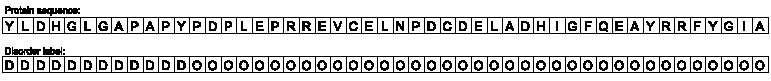
\includegraphics{images/groundtruth.pdf}    

    \caption{The Osteocalcin protein \citep{uniprot:22} and its disorder label. This ground truth label, represents disordered amino acids with a D and ordered amino acids are represented with O. Here we see the disordered region is at the start of this small protein sequence}

    \label{fig:groundtruth} 
\end{figure}

Compared to other problems solved by deep neural networks, such as protein structure prediction \citep{Jumper:21}, classifying images \citep{Xie:17} and language modelling \citep{Devlin:18}, the size of our manually labelled dataset is much smaller. Disprot only contains around 2500 protein sequences. However, we are not classifying an entire sequence as either ordered or disordered, we are classifying a single amino acid within the sequence as ordered or disordered as seen in Figure \ref{fig:groundtruth}. This is because we know the region of the protein can be disordered due to the characteristics of the grouped amino acids. This gives us sufficient labelled data. Using these labelled sequences as our ground truth, we can utilise our deep neural networks to recognise patterns and relationships about the amino acid sequence that causes intrinsic disorder in proteins through our supervised learning approach.

\section{Approaches}

Machine learning algorithms cannot operate on our protein sequences directly. Therefore, to ensure our model is equipped to handle the various amino acids, we will consider them as distinct categories of data and employ feature encoding techniques to generate a suitable numerical input \citep{Kumar:20}.

\subsection{One-hot}

Our first feature encoding approach is one-hot encoding \citep{One-hot:wiki} \citep{Fawcett:21}. We can treat each amino acid as a vector by using the one-hot encoding technique. Our vectors will have a size of 20 because of the twenty possible amino acids, therefore as these feature vectors are not excessively large, this one-hot approach is suitable. This has let us transform a raw amino acid sequence into a feature matrix, of shape $20 \times sequence length$, which now represents the sequence.

\subsection{Position-Specific Scoring Matrix (PSSM)}

Our other feature encoding approach is to generate a position-specific scoring matrix (PSSM) \citep{PSSM:wiki}. This technique is used in many protein structure problems, such as predicting protein secondary structure \citep{McGuffin:00}, identifying sequence-contact relationships \citep{Wang:17} and used within current approaches previously discussed in our review of the literature. A PSSM is a “matrix that involves information about the probability of amino acids or nucleotides occurrence in each position, which is derived from a multiple sequence alignment” \citep{Mohammadi:22}. These PSSMs provide an informative representation about the amino acids at positions within the protein sequences. Specifically, PSSMs capture information about the evolution of the protein in terms of which amino acids can occur at different positions in the sequence and this is used to determine whether a specific residue position will be a small amino acid, a bulky amino acid, a negatively charged amino acid, or have any other specific amino acid property. This information will be helpful for our network to identify patterns and relationships within protein sequences. Furthermore, as PSSMs are also of shape $20 \times sequence length$, the neural network models will be able to take both one-hot encoded sequence matrices and PSSMs as input without any changes, allowing us to compare these different feature encoding methods.

\section{Architectures}

\section{Evaluation metrics}
\label{chap:analysis sec:evaluation}
With our trained deep neural network, we will evaluate its predictions using similar approaches to the literature. As this is a binary classification task classifying amino acids as either ordered or disordered we can define our outcomes as: 

\begin{itemize}    
    \item True positive (TP): When the model correctly predicts that a disordered residue is disordered.
    \item True negative (TN): When the model correctly predicts that an ordered residue is ordered.
    \item False positive (FP): When the model incorrectly predicts that an ordered residue is disordered.
    \item False negative (FN): When the model incorrectly predicts that a disordered residue is ordered. \citep{google_TP}
\end{itemize}

By computing these outcomes, we can evaluate the accuracy, precision, recall (sensitivity) and specificity of our model. These metrics are widely used in various machine learning tasks as standard performance measures \citep{BC:wiki}. We can also calculate the F1-score which is the harmonic mean of the precision and recall and is another useful measure of how accurate our model is. Furthermore, as our dataset is imbalanced, with a majority of ordered labels, we will consider the Matthews correlation coefficient (MCC). This metric is a more reliable measure when dealing with an imbalanced and disproportionate dataset \citep{Chicco:20}.

With these evaluation metrics we will be able to compare our approaches and architectures against each other. We can also compare our models to known current approaches using the CASP datasets which have been used for benchmarking these protein disorder prediction models \citep{casp}.

\section{Django server}

In addition to evaluating deep learning models, it is necessary to create a Django-based server that enables users to submit a protein sequence and obtain a comprehensible representation of the disordered regions of the protein. From the literature, papers proposing protein disorder prediction tools also often set up an online server so their tool can be used such as UCL's PSIPRED workbench \citep{Jones:19} and the recently published Metapredict server \citep{Metapredict:server}. These protein prediction servers are important as they allow researchers to easily access these tools, allowing them to understand the structure and function of proteins which is useful for protein engineering \citep{prot_engineering:wiki}. 

A brief analysis of the server’s requirements are stated below; following the MoSCoW prioritisation method \citep{moscow}: 
\label{chap:analysis sec:moscow}
\subsection{Functional requirements}

\begin{itemize}    
    \item Must have: The server will have a web interface, so it is easily accessible for use by researchers.
    \item Must have: Users can submit a single protein sequence via a form.
    \item Must have: The server can make a prediction on a protein sequence using a deep neural network. This model will be chosen from our evaluation.
    \item Should have: The web interface will have a clear visualisation displaying the sequence to the user with clearly identified IDRs.
    \item Could have: The web interface will have a graphical representation of the identified IDRs.
    \item Will not have this time: The visualisation of the disordered sequence cannot be saved.
    \item Will not have this time: The server will not allow multiple sequences to be entered in a single form submission.
\end{itemize}

\subsection{Non-functional requirements of our server}

\begin{itemize}    
    \item Must have: The web interface will be intuitive and easy to use. Both when entering information in via the form and interpreting the outputted sequence with highlighted disordered regions.
    \item Should have: The web application should be containerised to follow best practices and be easily portable.
    \item Could have: The Django server could interact with an external database for efficient lookup of previously entered sequences and their representations.
    \item Will not have this time: The web page will not be hosted and accessible via a searchable domain by the conclusion of the project.
\end{itemize}



%==================================================================================================================================
\chapter{Design}
\label{chap:design}

\section{Data processing}

We will need to build a data processing pipeline where we will gather specific information about each unique protein from the DisProt dataset, such as their full sequence and the location of all the disordered regions, so we can create our ground truth label. This ground truth label is vital for our supervised learning task. Given our DisProt dataset, we identify unique proteins using a UniProt accession identifier. Therefore, we should use this accession identifier as a key in hash map data structures. This will let us easily lookup the feature encoded sequence for our DNN's input and a sequence’s true disordered regions which let us create our label for evaluating our prediction. We build the label by creating a vector the size of the sequence, and from our looked up disordered regions of a given protein we will set the amino acids where intrinsic disorder occurs to 1 (as disorder is our positive class) and ordered amino acid positions will be set to 0. This vector will be used in our loss function which is discussed later in Section \ref{sec:loss design}. 

Processing is also required to encode these sequences before they are looked up. We have two different vectorised representations of these sequences: a one-hot encoded matrix and a PSSM. The one-hot encoded matrix is a sparse matrix and is made using standard one-hot feature encoding. An example of the beginning of a one-hot encoded sequence is shown in Figure \ref{fig:feature encoding}. The generation of the PSSMs is more computational than the one-hot encoding and involves using a sequence alignment search tool alongside a large protein sequence database. This processing gives us information about the conservation of amino acids between similar sequences which conveys more information about the sequence than a one-hot representation. An example of a PSSM is shown in Figure \ref{fig:feature encoding}, and each PSSM can be parsed into a 2D data structure which creates the appropriate matrix format our deep neural network can use. A limitation of using PSSMs is that they are much more computationally expensive to create than our one-hot encoding approach as they perform sequence alignment using a very large protein database such as UniProt \citep{uniprot:22}. For this reason, we have also implemented a one-hot encoding approach to see if generating PSSMs is worth the computational expense. 

\subsection{Training, validation and testing data}
\label{chap:design section:datasets}

Our final key processing step is to divide our dataset into a training, validation and test set before any learning takes place. We follow the common approach of using 20\% withheld data for the test set, and the rest will be used for training and validating the model. We will further separate this training and validation set by 75\% and 25\% respectively so that the overall split of training, validation and testing data is 60\%, 20\% and 20\% respectively. Random sampling (with a seed to ensure reproducible splitting) will be done to separate these sequences. However, as protein sequences can have a similar ancestor, this means they can be homologous and there may be data leakage between datasets. This means information from the test dataset can accidentally appear in our training dataset \citep{Cook:22}. To detect this data leakage, we will look for homologous sequences by employing a homology clustering search. We will avoid any data leakage by moving sequences between datasets if they are homologous, such that all datasets will not have homologous sequences between them. Despite movement of sequences, we still aim to have a division of approximately 60\%, 20\%, 20\% between our three datasets and will verify this before we perform further evaluation. 

\begin{figure}[!ht]
    \centering
    \begin{subfigure}[h]{0.45\textwidth}
        \centering
        \caption{One-hot encoding}
        \label{fig:feat1}
        \begin{tabular}{|c|cccccc|}
        \hline
          & M & A & S & R & E & ...\\ \hline
        A & 0 & 1 & 0 & 0 & 0 & \\ 
        C & 0 & 0 & 0 & 0 & 0 & \\ 
        D & 0 & 0 & 0 & 0 & 0 & \\ 
        E & 0 & 0 & 0 & 0 & 1 & \\ 
        F & 0 & 0 & 0 & 0 & 0 & \\ 
        G & 0 & 0 & 0 & 0 & 0 & \\ 
        H & 0 & 0 & 0 & 0 & 0 & \\ 
        I & 0 & 0 & 0 & 0 & 0 & \\ 
        K & 0 & 0 & 0 & 0 & 0 & \\ 
        L & 0 & 0 & 0 & 0 & 0 & ...\\ 
        M & 1 & 0 & 0 & 0 & 0 & \\ 
        N & 0 & 0 & 0 & 0 & 0 & \\ 
        P & 0 & 0 & 0 & 0 & 0 & \\ 
        Q & 0 & 0 & 0 & 0 & 0 & \\ 
        R & 0 & 0 & 0 & 1 & 0 & \\ 
        S & 0 & 0 & 1 & 0 & 0 & \\ 
        T & 0 & 0 & 0 & 0 & 0 & \\ 
        V & 0 & 0 & 0 & 0 & 0 & \\ 
        W & 0 & 0 & 0 & 0 & 0 & \\ 
        Y & 0 & 0 & 0 & 0 & 0 & \\ \hline
        \end{tabular}
    \end{subfigure}
    \begin{subfigure}[h]{0.45\textwidth}
        \centering
        \caption{Position-specific scoring matrix}
        \label{fig:feat2}
        \begin{tabular}{|c|cccccc|}
        \hline
        & M & A & S & R & E & ...\\ \hline
        A & $-2$ & $\phantom{-}4$ & $\phantom{-}0$ & $-2$ & $-1$ & \\
        C & $\phantom{-}0$ & $\phantom{-}0$ & $\phantom{-}0$ & $-2$ & $-2$ & \\
        D & $-3$ & $-2$ & $\phantom{-}0$ & $-1$ & $\phantom{-}0$ & \\
        E & $-4$ & $-3$ & $-2$ & $-1$ & $\phantom{-}4$ & \\
        F & $\phantom{-}1$ & $-1$ & $-1$ & $-2$ & $-2$ & \\
        G & $-3$ & $\phantom{-}0$ & $-1$ & $-2$ & $-2$ & \\
        H & $-2$ & $-2$ & $-2$ & $-1$ & $-1$ & \\
        I & $\phantom{-}2$ & $\phantom{-}0$ & $-1$ & $-2$ & $-2$ & \\
        K & $-2$ & $-2$ & $-1$ & $\phantom{-}0$ & $\phantom{-}0$ & \\
        L & $\phantom{-}3$ & $\phantom{-}0$ & $-1$ & $-1$ & $-2$ & ... \\
        M & $\phantom{-}7$ & $-1$ & $-1$ & $-1$ & $-2$ & \\
        N & $-3$ & $-2$ & $\phantom{-}0$ & $-1$ & $-1$ & \\
        P & $-3$ & $-1$ & $-1$ & $-2$ & $-2$ & \\
        Q & $-2$ & $-2$ & $-2$ & $\phantom{-}2$ & $\phantom{-}0$ & \\
        R & $-3$ & $-4$ & $-3$ & $\phantom{-}3$ & $-2$ & \\
        S & $-3$ & $\phantom{-}0$ & $\phantom{-}4$ & $-2$ & $\phantom{-}0$ & \\
        T & $-1$ & $-1$ & $\phantom{-}0$ & $-2$ & $-1$ & \\
        V & $\phantom{-}1$ & $\phantom{-}0$ & $-1$ & $-2$ & $-1$ & \\
        W & $\phantom{-}0$ & $-1$ & $-1$ & $-1$ & $-2$ & \\
        Y & $\phantom{-}0$ & $-1$ & $-1$ & $-1$ & $-1$ & \\ \hline
        \end{tabular}
    \end{subfigure}
    \caption{Two possible ways of encoding our protein sequences. \subref{fig:feat1} shows a one-hot encoding approach, where 1.0 identifies the amino acid at each sequence position. \subref{fig:feat2} shows the PSSM, where larger positive values are given to amino acids that are expected to appear at each position of the sequence. This protein is Human adenovirus C serotype 5 (HAdV-5) (Human adenovirus 5), the first protein sequence in the DisProt dataset, and we show the first five amino acids from this sequence.
    }\label{fig:feature encoding}
\end{figure}

\section{Our neural networks and how we train them}

\subsection{Model input}

Giving the model input is the initial stage in training a DNN. The input to our models will be our feature encoded sequence (either a one-hot or position-specific scoring matrix), which will have shape $20\times sequence length$. We will only give a model one protein sequence to evaluate at each forward pass as we know that sequence lengths differ between proteins; therefore, we cannot batch multiple sequences together. Batching multiple sequences would create an unexpected, irregular shape, which neural network layers cannot handle. Thus, we use a batch size of one as input to our DNN models.

\subsection{CNNs}
\label{chap:design section:cnn}

Our CNNs must actually be fully convolutional neural networks (FCNs) because our protein sequences have different lengths, therefore we cannot use a fully connected layer as it expects a fixed size tensor \citep{fcn_seg}. So, we will only use convolution layers which create feature maps for our model to identify information about the protein sequences used for the disorder classification task. These layers must also reshape our input to a $1\times sequence length$ length tensor for our loss function.

There are two different convolutional neural networks we can design: one that treats our protein sequence as a black and white image and uses 2D convolutions, or one that treats each row in the encoded matrix (different amino acids) as a different feature representation of the input sequence and uses 1D convolutions over these separate feature input channels. 

\subsection*{Using 2D Convolutions}

Usually, a 2D convolutional kernel is applied to images, therefore given our $20\times sequence length$, the height of the proposed image is the number of possible amino acids, and the width of the image is determined by the sequence. Our input to a CNN using 2D convolutions must follow the [batch size, channels, height, width] constraint, therefore our input will be a tensor of shape [1, 1, sequence length, 20] due to batching of size 1 and treating the colour channel as black and white. 

As discussed earlier, we want our convolution kernel to behave like a sliding window (Section \ref{chap:background sec:litrevCNN}), therefore it must overlay the entire height of the image to take in a full context window of amino acid information. Capturing the entire height involves using a kernel of size 20, however we cannot appropriately pad the width of the sequence with this kernel shape such that the same width is returned after convolving with a kernel of this shape. The width cannot be changed as it is necessary to compare each amino acid disorder classification against its true label. Therefore, we will use a non-square convolution kernel so that the width of our kernel is an odd value and appropriate padding can be included. 

After the first convolution layer, layers after this will be dependent on the feature map created by this first layer and further layers. The number of feature channels produced by this first convolution layer can be experimented with and we have chosen to use ten hidden channels. After further convolution layers we want our final feature map output to take shape $1\times sequence length$ so our predictions can be compared against the true label. 

\subsection*{Using 1D Convolutions}

Our other fully convolutional network uses 1D convolutions. Usually, a 1D convolution kernel is applied to sequences and accepts an input of $1\times sequence length$ shape. For our neural network, we will treat each amino acid feature representation as a separate input channel, giving us 20 channels, each with shape $1\times sequence length$. The input to the model must follow the [batch size, input channels, width] constraint, therefore our input will be a tensor of shape [1, 20, sequence length]. This 1D convolution kernel also behaves like a sliding window, and a kernel will produce one output feature map which represents all the amino acid input channels. This ensures all amino acid information is captured for a context window at each position along the sequence. Furthermore, an odd numbered kernel must be chosen so that appropriate padding can be included to the width of our sequence similarly to the 2D CNN. Like the 2D CNN, all further convolution layers can be changed within the network as long as the final layer produces a $1\times sequence length$ feature map as its output for comparison with our ground truth labels.

\subsection{RNN}
\label{chap:design section:rnn}

Our RNNs will use the long short-term memory (LSTM) architecture. These LSTMs combat the vanilla RNN’s vanishing gradient problem, and they can identify long-term dependencies which we know is useful from our literature analysis. Usually, LSTMs are applied to sequential data, and they expect a batch size, a sequence length and a number of feature channels. These features are represented in the same way as our 1D CNN initial feature channels; where each amino acid row from our vectorised protein sequence is used to represent the sequence as a separate feature vector. As using batching requires our sequences to be the same length, which we do not have, we will continue to batch with a single sequence in each batch instead of padding our sequences. Therefore, our input to the LSTM model will be a tensor of shape [1, sequence length, 20]. 

We also need to initialise our hidden state for our LSTMs. These will be initialised with all zeros every forward pass, so they are reset each sequence. It is common practice to set the hidden state to an all zero tensor with a shape considering the batch size and the number of hidden dimensions we want. In our model we will choose to have 32 hidden dimensions. 

Finally, our LSTM will be a bidirectional LSTM (BLSTM). This performs better than a traditional LSTM and can capture long-term dependencies about the IDPs using information from the start and end of these sequences. With information flowing in both directions, we can capture more contextual information about each amino acid. Furthermore, a protein sequence does not have a flow of information like a time series, and the start (N-terminus) and end (C-terminus) of a sequence is chosen arbitrarily, meaning this protein could be written in the opposite direction. Thus, it is useful to assess each sequence from both directions. A limitation of implementing a bidirectional network is that it will be much slower to compute because forward propagation requires both forward and backward recursions, which creates a long dependency chain and affects our gradient calculation using backpropagation \citep{Zhang:2021}.  

Like our other networks, our LSTM will use a final linear layer to reduce our feature map down to a single feature (the disorder classification), so that a $1\times sequence length$ output is returned for the rest of our training loop to handle.

\subsection{Activation functions}
\label{chap:design section:activations}
Between each layer in our neural networks, we use the rectified linear unit activation function (ReLU) as it is “the most widely used and a goto activation function for most types of problem,” \citep{Keerthi:22}. This is because ReLU can be more computationally efficient than other activation functions, and using ReLU in networks tends to give a better convergence performance \citep{BerenLuthien:16}. After our final layer, we employ the sigmoid activation function because this gives us a value in the range [0, 1]. We can treat this value as a probability as it shows how likely that this position in the sequence is a disordered amino acid. This value alongside a threshold of 0.5 will be used to identify the predicted IDRs; where any position with a value greater or equal to 0.5 can be regarded as disordered. Furthermore, these probability values can be evaluated under various thresholds, letting us assess the effectiveness of our models, which is further discussed in our design of the evaluation (Section \ref{chap:design sec:evalThresh}).

\section{Discussion about loss function and optimisation}
\label{sec:loss design}
To allow our deep neural network to learn and update its many different weights in each layer, we must use an optimisation method and an appropriate cost function. We know our problem is a binary classification task from our analysis of the problem; therefore, we can use binary cross-entropy (also known as log loss) as our loss function \citep{Godoy:18}, shown in Figure \ref{fig:bceloss}.  

With these two possible outcomes we are treating a disordered amino acid as the positive class and an ordered amino acid as the negative class. From analysing our DisProt dataset, we see that our two classes are imbalanced: there are a lot more ordered amino acids within these intrinsically disordered proteins, specifically there are approximately five ordered amino acids for every disordered amino acid. One way of handling this imbalanced dataset is using a weighted loss function. For this, we calculate the number of ordered and disordered amino acids in our training dataset. Then, we can calculate a weight multiplier to be used to give the disordered amino acids loss more weighting. By scaling the loss of predictions about the amino acids we will emphasise predictions that should take a disordered label which will help the model better identify this disproportionate class because the model will be penalized more heavily for misclassifying disorder. 

This binary cross-entropy loss function is useful for gradient-based optimisation algorithms because it is easy to compute and is sensitive to small changes in the predicted probabilities. We plan to use stochastic gradient descent (SGD), which is a popular machine learning optimisation algorithm. We will also experiment using the Adam optimiser, however as this optimisation method usually works well with large datasets and SGD is known to generalise better than Adam \citep{Zhou:20}, I believe SGD will be a better optimisation method and produce a better model. 

\begin{figure}[h]
    \centering
    \begin{equation}
    \ell(y, \hat{y}) = -\frac{1}{N} \sum_{i=1}^{N} w_i [ y_i \log(\hat{y}_i) + (1-y_i)\log(1-\hat{y}_i)]
    \end{equation}
    \caption{Binary Cross-Entropy (Log Loss) Function. This equation represents the loss function used in binary classification tasks. For our task, $y$ is the true label of order or disorder, $\hat{y}$ is the predicted probability (i.e., the output of the sigmoid function), and $N$ is the number of amino acids in the sequence. The function measures the difference between the predicted and true labels. The weight vector $w$, is used to penalise the model more when it is more certain about incorrect predictions of the disordered class. Having an all ones vector for $w$ is default when no weights are specified.}
    \label{fig:bceloss}
\end{figure}

\section{The design of our evaluation experiments}
\label{chap:design sec:eval}

During the training of our model, we will evaluate the performance of the optimisation task. We can use the total loss of our training set and validation set predictions to ensure our model is learning at a sufficient rate and is generalisable on withheld data. Using the validation dataset as our first withheld dataset, we can optimise hyperparameters, such as the learning rate and regularisation weights to make sure our validation loss decreases along with our training loss. Furthermore, we will plot loss curves to make it visually clear our model is generalisable to our validation dataset \citep{Brownlee:19}. With a generalisable model we are more likely to achieve correct classifications on future unseen data. 

After tuning the important hyperparameters for our different model configurations we will retrain our model using the 80\% of the DisProt dataset allocated to training data (this includes our training and validation datasets). Using the other 20\% of the DisProt dataset withheld for testing, we will evaluate our models using the evaluation metrics discussed in our analysis (Section \ref{chap:analysis sec:evaluation}). Discussion about these metrics and the equations for these standard machine learning evaluation measures are given below. 

\begin{equation*}
Accuracy = \frac{TP + TN}{TP + TN + FP + FN} ,
\end{equation*}
where TP (true positives) is the number of correctly classified disordered amino acid instances, TN (true negatives) is the number of correctly classified ordered amino acids instances, FP (false positives) is the number of incorrectly classified disordered amino acids instances, and FN (false negatives) is the number of incorrectly classified ordered amino acids instances.

\begin{equation*}
Precision = \frac{TP}{TP + FP} ,
\end{equation*}
Precision measures the proportion of amino acids classified as disordered among all disorder predictions.

\begin{equation*}
Recall = \frac{TP}{TP + FN} ,
\end{equation*}
Recall measures how many disordered amino acids are actually detected among all actual disordered amino acids.

\begin{equation*}
Specificity = \frac{TN}{TN + FP} ,
\end{equation*}
Specificity measures the proportion of amino acids classified as ordered among all order prediction instances.

\begin{equation*}
F1\ score = \frac{2 \times Precision \times Recall}{Precision + Recall} ,
\end{equation*}
F1 score is the harmonic mean of precision and recall and this provides a balanced measure of both these metrics.

\begin{equation*}
MCC = \frac{TP \times TN - FP \times FN}{\sqrt{(TP + FP)(TP + FN)(TN + FP)(TN + FN)}}
\end{equation*}
MCC considers all four confusion matrix elements. It ranges from -1 to 1, with 1 indicating a perfect correlation, 0 indicating no correlation, and -1 indicating a perfect negative correlation.

\subsection{Evaluation of classification thresholds}
\label{chap:design sec:evalThresh}

Finally, we consider the probability-based values returned from our sigmoid activation function in our evaluation. In a binary classification task, classifying the positive class can be imperative, such as cancer detection where false negatives could lead to delayed diagnosis and missed treatment opportunities. \cite{Ardila:19} agree that classifying the positive class can be critical with their production of a DNN for lung nodule detection. In some scenarios, it may be more important to predict every disordered amino acid correctly than it is to misclassify more ordered amino acids. However, for our evaluation it is important our model still behaves sensibly. To assess a model's capability at predicting disordered amino acids correctly, we can use receiver operating characteristic (ROC) curves and the area under the ROC Curve (AUC). This lets us determine what an appropriate threshold for identifying disorder can be and if our models perform better than a dummy classifier that predicts blindly.

\subsection{Evaluating on different datasets}
After our full evaluation is complete, we will finally train our model using all (100\%) of our data from the DisProt database as the separate datasets have served their purpose in helping us find the best model. Training with this extra data means that our model should have at least the performance accuracies as it did in our evaluation, and this is a best practice before deploying a machine learning model \citep{Brownlee:17}. After this step, our trained model is ready to be deployed on our web server and can be assessed using other unseen datasets. 

Furthermore, we will use the CASP10 dataset to evaluate our model. This dataset contains 94 protein sequences \citep{Moult:14} and has been used to assess many protein disorder classifiers. Details of other protein disorder prediction methods performances can be found in other papers; therefore, we can compare our findings against other approaches and architectures. 

\section{The web server}

\subsection{User interface}

The user interface was designed to be similar to other protein disorder prediction websites. All websites used an input form, stated what input was valid and displayed the output to the user in a timely manner for single sequences. From checking popular protein prediction web servers, I felt the most user-friendly websites included an example of what sequence input was valid, therefore I made this a consideration when building the website. 

We have two pages on our web server: the input form and the displayed disorder prediction.

\subsubsection{The input form web page.}

This page was made to be intuitive, and its main feature is a form to let the user input a protein sequence. This satisfies must have functional requirements for the web server (Section \ref{chap:analysis sec:moscow}). The input to this form can only be a valid protein sequence or FASTA file, which is explained on the web page. We have also included links to PDB, UniProt and DisProt to assist users in finding protein sequences. The wireframe for this page is shown in Figure \ref{fig:wireframe1}.

\begin{figure}[!htb]
    \centering
    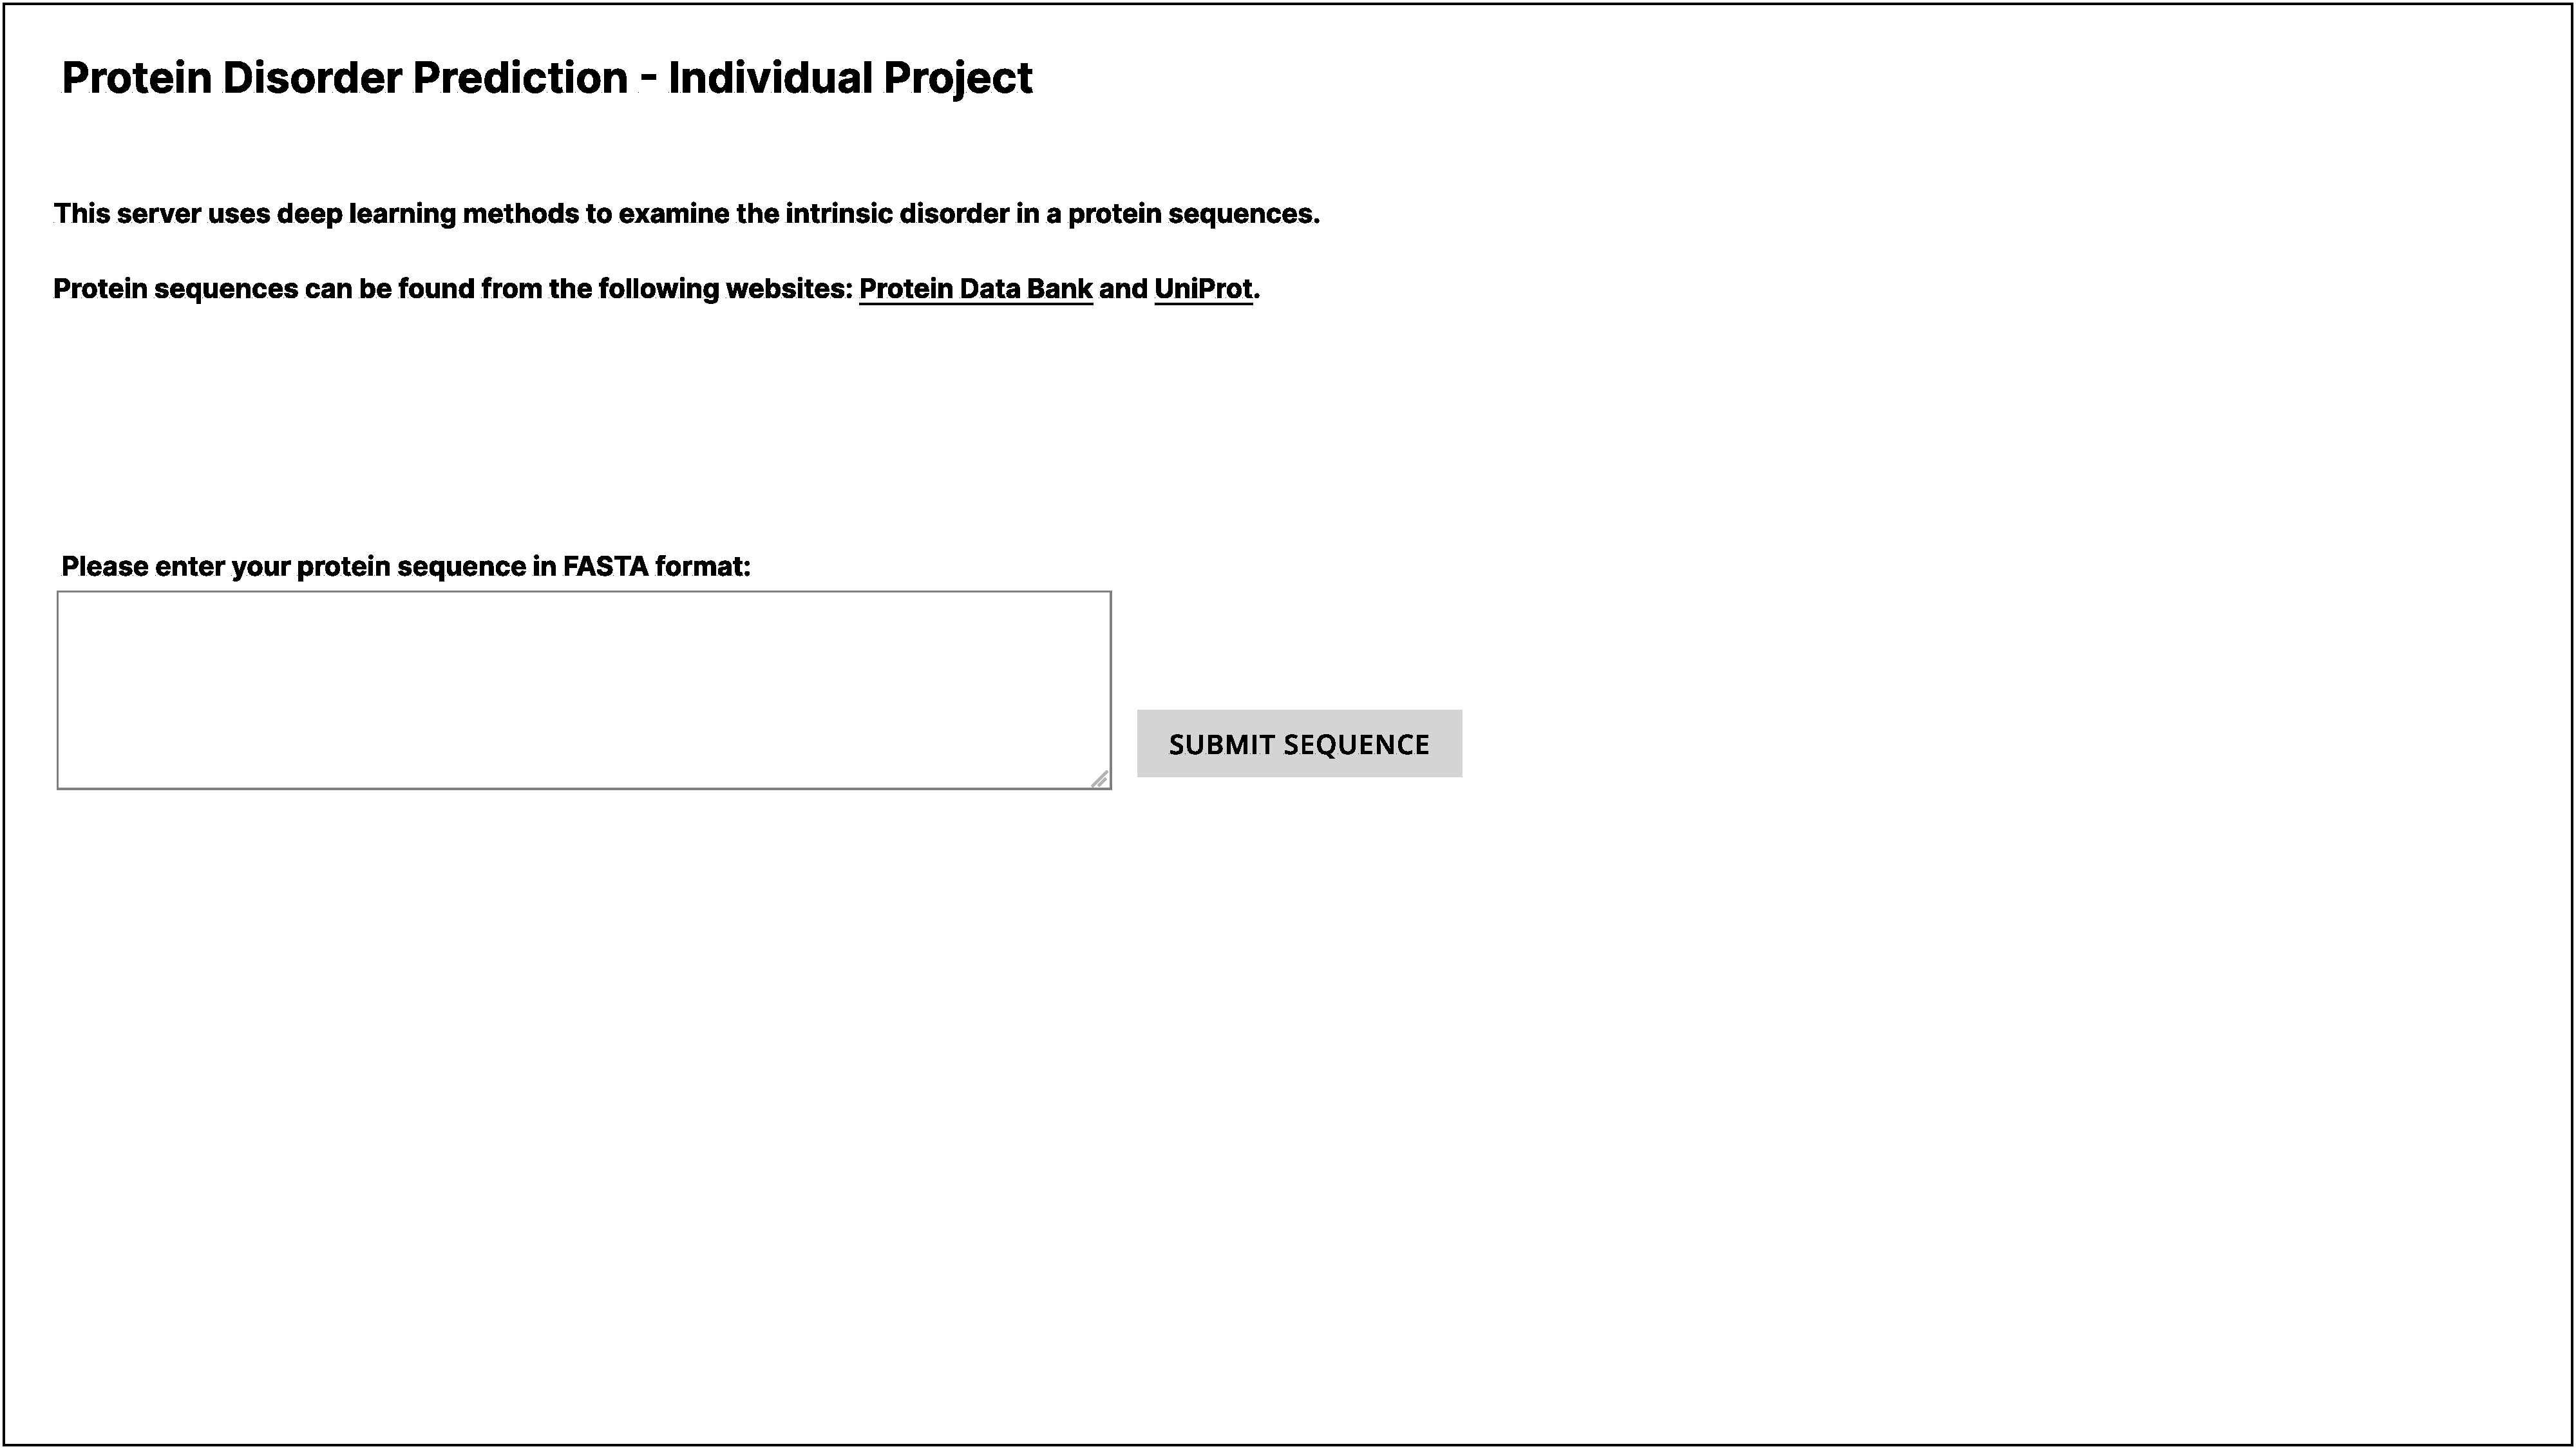
\includegraphics[width=\linewidth]{images/Index-forminput.pdf}
    
    \caption{The home page of our web server. This wireframe shows that users can navigate to external protein database websites, and enter their protein sequence in FASTA format to our input form.}
    
    \label{fig:wireframe1} 
\end{figure}

\subsubsection{The disorder prediction web page.}

This page displays the IDR predictions. We have used a sequence-based visualisation, which demonstrates which amino acids are disordered and where the disordered regions are. Other web servers such as ESpritz \citep{Walsh:11} have also used a sequence display, but this website is older and uses a ‘D’ or ‘O’ label next to the amino acid instead of a coloured label. We believe that the coloured approach is more effective at representing the disordered regions and has also been adopted by web servers that have been maintained and updated recently like PSIPRED \citep{Jones:19}. The wireframe of this page is shown in Figure \ref{fig:wireframe2}.

\begin{figure}[!htb]
    \centering
    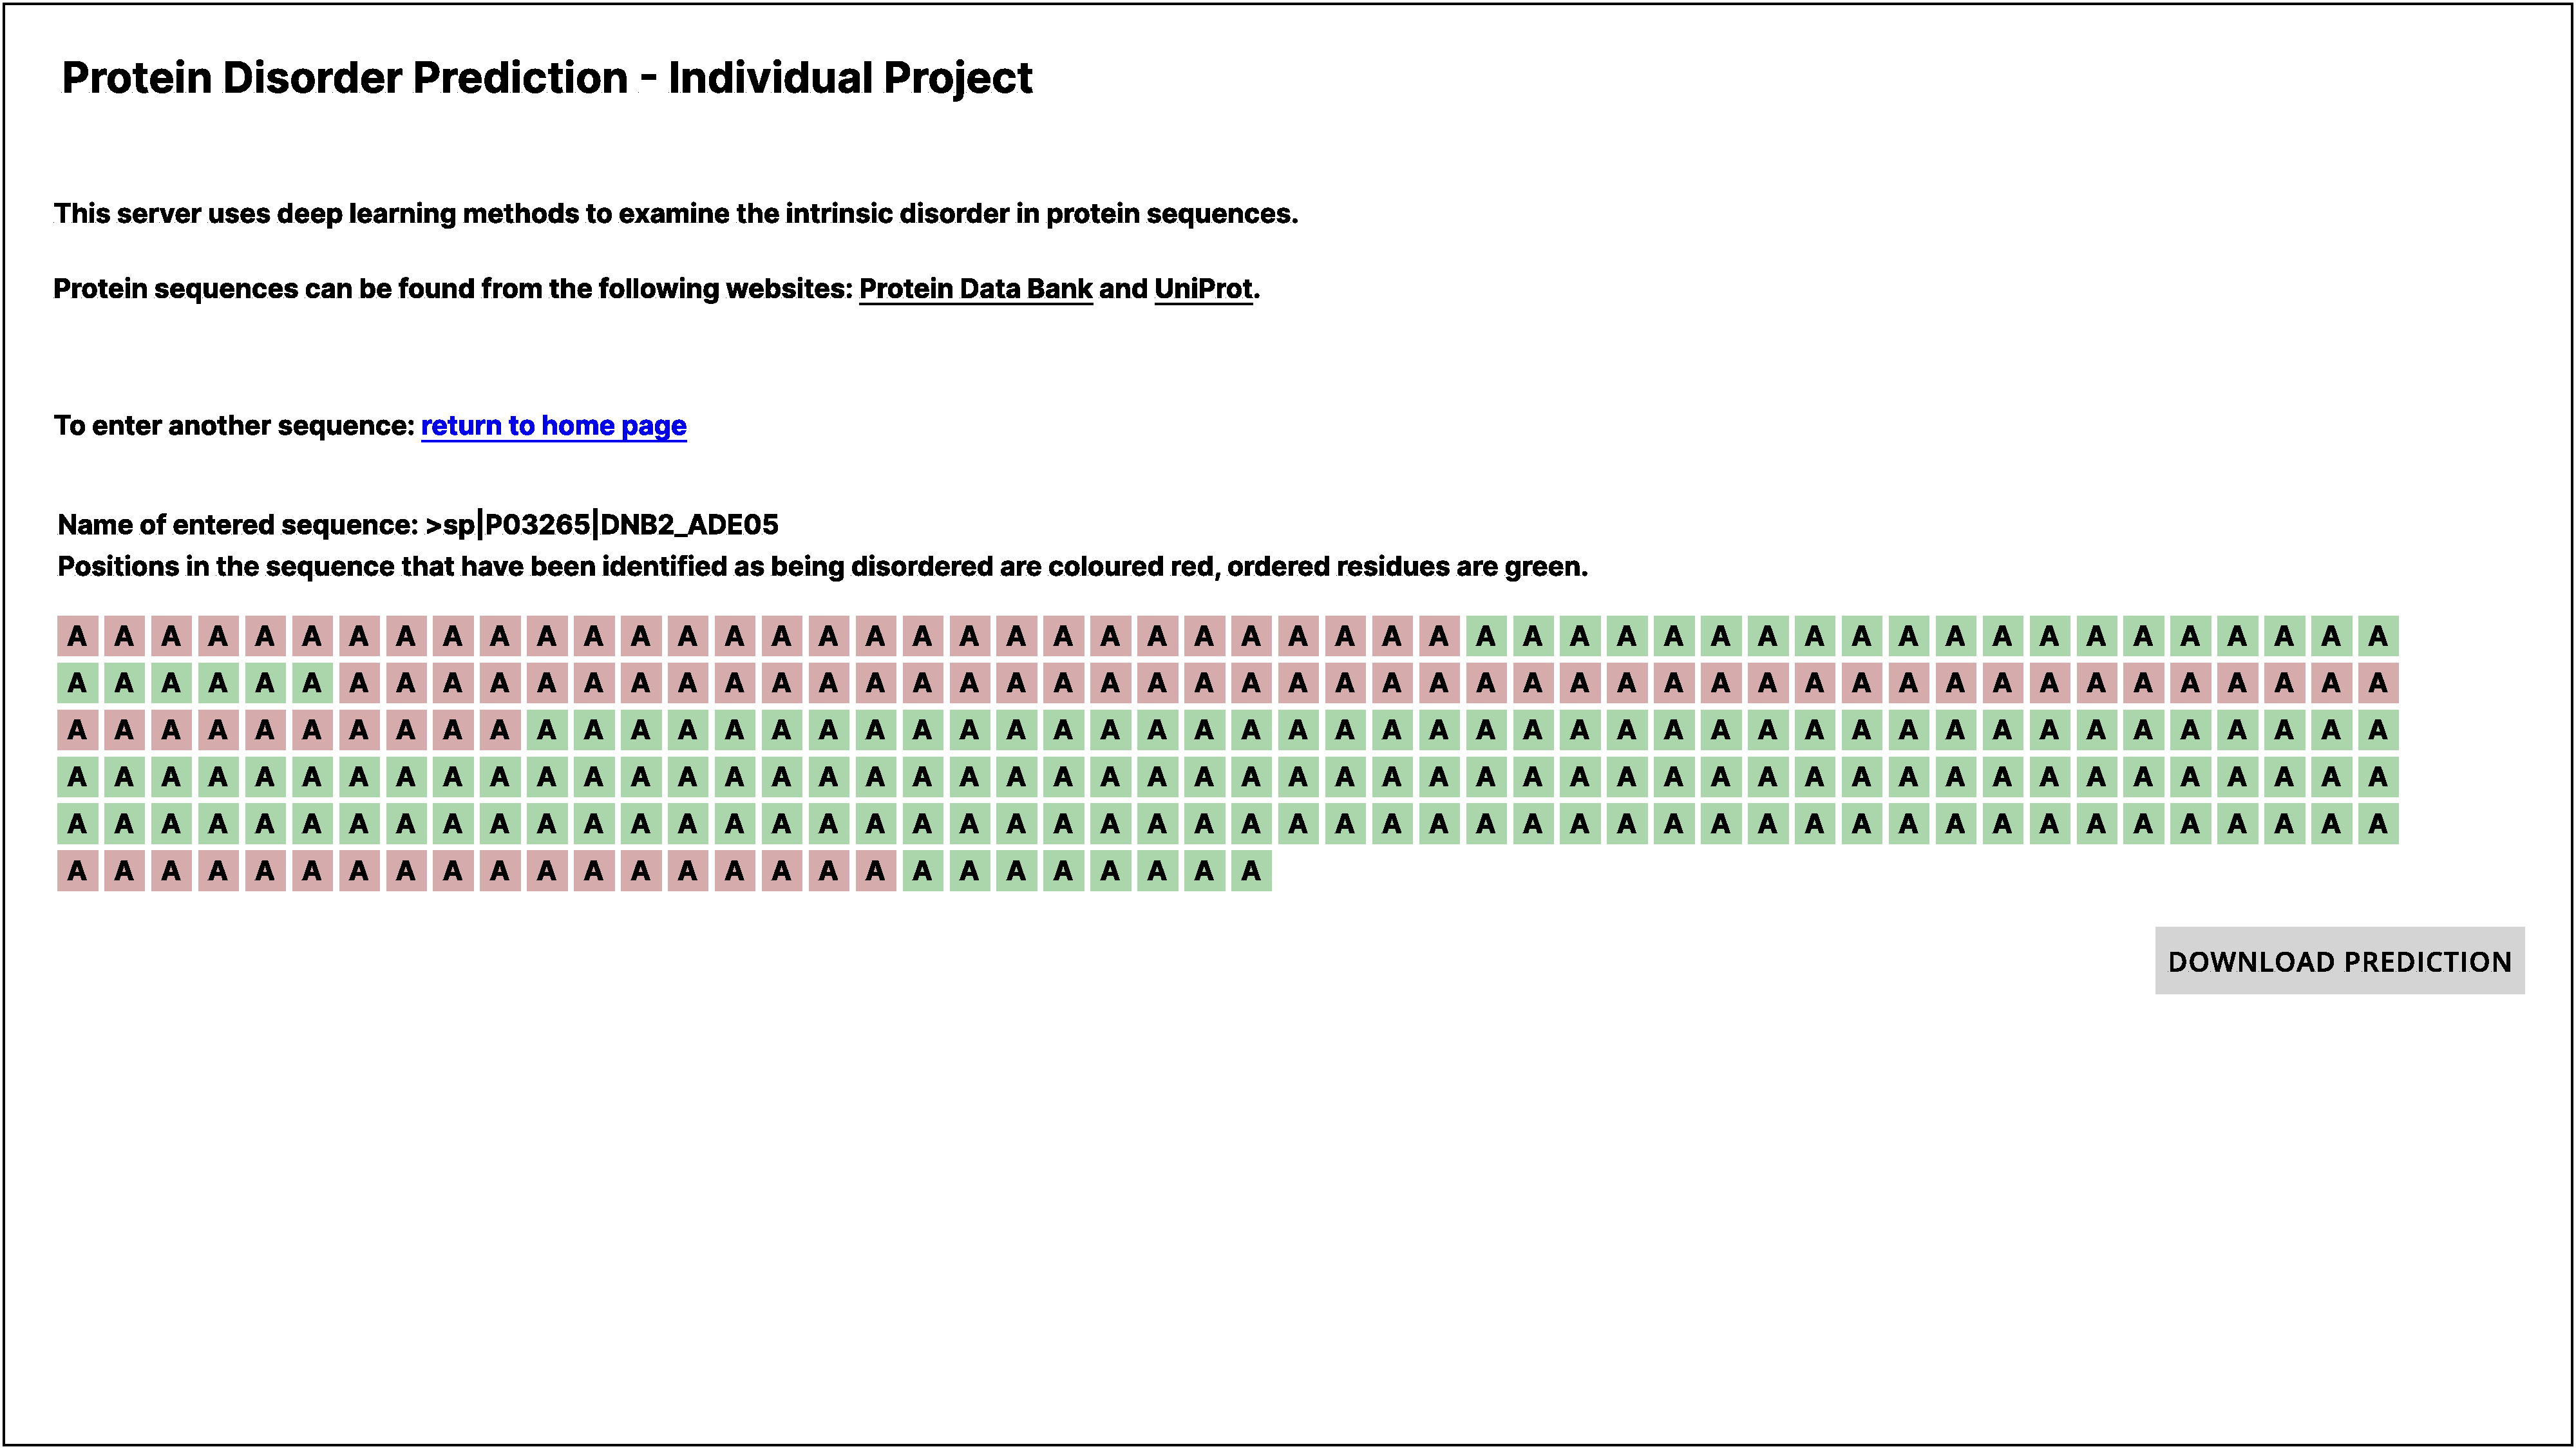
\includegraphics[width=\linewidth]{images/Index-disorderprediction.pdf}
    
    \caption{The disorder prediction web page. This wireframe demonstrates how our deep learning models classification of disordered regions will be displayed after a protein sequence has been submitted.}
    
    \label{fig:wireframe2} 
\end{figure}

\section{Tools and technologies}
It is important that the trained deep neural network model must be easily accessible on the web server. Using PyTorch for the deep learning and Django for the web server will allow us to integrate our trained PyTorch model into our web application easily, using Python for consistency.

\subsection{Deep learning}

To create our different deep neural network architectures, the PyTorch framework \citep{pytorch} was used. PyTorch lets us construct our models using their neural network library. Using Python also allows us to carry out our pre-processing and evaluation steps with different libraries that help us make efficient computations along with appealing and informative visualisations about the performance of our prediction task. Using Python also lets us utilise Google colab’s notebooks \citep{Bisong:19}, where we can use a GPU for decreased training times and include markdown throughout our notebook, which helps with the understanding of our code.

An external tool is required to generate the encoded features for our model's PSSM input. We have chosen to use MMSeqs2 (Many-against-Many sequence searching) \citep{Steinegger:17}. MMSeqs2 can perform multiple sequence alignment searches much faster than PSI-BLAST \citep{Altschul:97} and HHblits \citep{Remmert:12} which are other software suites used for PSSM generation. Despite HHblits giving slightly more accurate alignments, this task is much more computationally efficient with MMSeqs2, which still generates accurate alignments. Recent papers, such as NetSurfP-2.0 \citep{Klausen:19} have used MMSeqs2 to generate their PSSMs for large sequences due to MMSeqs2 being less resource intensive than HHblits and found little differences in the models' performance trained using PSSMs generated by the different suites.

\subsection{Web server}

To create our web server, we will use the Django web framework \citep{Django:05}. Web pages will be built using standard web technologies (HTML, CSS and JavaScript). In Django’s backend we will have the views which can process requests and manipulate the data as needed. We will save our trained neural network as a serialized PyTorch state dictionary, which is a Python dictionary that includes the weights, biases, and other model state variables for a PyTorch model. This saved model can be reloaded within the views of the Django backend so that the web application can make use of it. Furthermore, this should be straightforward to do as Django is a Python web framework, PyTorch can be easily imported and loaded amongst the web application logic. Finally, we have used Docker \citep{Docker:14} along with Nginx \citep{Nginx:08} and Gunicorn \citep{gunicorn:wiki}, so that our web server can be containerised and is portable which is one of our initial requirements. 

%==================================================================================================================================
\chapter{Implementation}

\section{Data processing}

\subsection{The IDPs}

Our data processing started with getting annotated disordered proteins and their disordered regions from DisProt \citep{disprot}. We used the DisProt dataset that was released in June 2022 (release 2022\_06) and kept the default settings that gave individual rows for each disordered region in a sequence, included ambiguous sequences and excluded obsolete sequences. We downloaded the TSV format of this file because it works particularly well with pandas \citep{Mckinney:10}, which we used at the start of our data processing stage. We stuck with this dataset throughout the entire project to maintain consistency in our experiments. To download this dataset, DisProt’s RESTful API search feature \citep{disprot} was used. We customised the request to match the terms given for the default settings on the main website and downloaded this file to our data folder. These terms can be modified, so that the most up to date dataset can be downloaded, processed and used to train and evaluate our models in the future.

DisProt only contained information about disordered regions, such as the start and end of these disordered regions, but not the consensus of all disordered regions for a given protein sequence or the full sequence itself. However, DisProt uses the UniProt accession identifier to identify proteins. Therefore, we grouped all disordered regions for a single identifier together, so they could be looked up to build a ground truth label. We also used these unique identifiers to make requests using UniProt’s REST API \citep{uniprot:22}, where we retrieve a sequence in FASTA format. We take the substring of the FASTA file, so that we just have the sequence. During these pre-processing stages we found that some protein sequences have been deprecated from UniProt (as it is updated more regularly than DisProt). To ensure extensibility of this processing stage we remove proteins from our DisProt dataset if the UniProt REST API identifies them as deprecated. This did not have an impact on the size of the dataset; we removed three protein sequences. Furthermore, we also remove sequences that are returned by UniProt with ambiguous amino acids. This is because these amino acids were not recognised in the list of twenty known amino acids and our vectorisation feature encoding cannot handle these unknown characters. This also has no effect to our dataset; we removed a further seven protein sequences.

Overall, this first processing stage of the IDP data from DisProt has produced two important data structures we needed: a map to all of our disordered protein sequences, and a map to all of our disordered regions for each protein. These are both connected via an accession identifier.





\subsection{Feature encoding}
\label{chap:implementation sec:features}

The next data processing step is performing feature encoding steps, so that a deep neural network can use protein sequences as input. With the one-hot encoding approach: for each sequence, if the amino acid at a position is present, then that amino acid row is given a 1 at that position, and all other amino acids are given a 0 at that position. This was done in Python, where we manipulated all zero NumPy arrays, and updated the amino acid at this position with 1 using a look up dictionary that let us access the feature vector representing that amino acid. Finally, all of these feature vectors were combined to create the full one-hot encoded matrix. For our PSSM approach: we first used the MMSeqs2 software suite \citep{Steinegger:17}, then cleaned the generated PSSMs so they are numerical tensors. Using MMSeqs2 required a protein database, so we used the UniProtKB, which is assembled of both UniProtKB/Swiss-Prot and UniProtKB/TrEMBL \citep{uniprot:22}. A FASTA file of all of the protein sequences was required, so we created this using the UniProt REST API. We did not modify our sequence string and wrote the full FASTA to an external file. This ensured PSSMs would only be generated for the sequences we had validated. Finally, we performed the multiple sequence alignments (MSAs) on these sequences with the downloaded database. All of these sequences were in the same FASTA file, meaning MMSeq2’s powerful scalability could be utilised. From the MSAs we can generate our PSSMs using MMSeq2’s tools. Finally, these are converted to a 2D tensor using Python’s string splitting functionality. For both of our feature encodings, we pair the numerical representation of the sequence with its accession identifier. This lets us quickly access our feature encoded sequences.

\subsection{Separating datasets}

For our training, validation and testing datasets we randomly sampled sequences using a seed so that this experiment can be repeated. The design discussed problems with our datasets (Section \ref{chap:design section:datasets}), so we cannot have sequences homologous to each other in different datasets. To find these homologous sequences we used MMSeqs2 clustering functionality \citep{Steinegger:17}. We already have our training, validation and testing dataset splits; therefore, each sequence was tagged with the dataset it was in. By examining these sequences using similarity clustering between sequences we can identify which sequences are homologous to each other. We found there was 286 sequences that have homologies with sequences from other datasets, therefore our datasets were not independent. To establish independence and ensure sequences that are related to each other did not overlap different datasets, we moved these flagged sequences from their dataset to the dataset the similar, homologous sequence is in. An example of this is shown in Table \ref{tab:MMSeqs clustering}. This removed the issue of leaking data. From these separated accession identifiers, three lists were created for the train, validation and test set. Using these lists of accession identifiers, we could get the sequences, ground truth labels and encoded features for any of our datasets as the unique accession identifiers are the key element to looking up all these pre-processed items.

\begin{table}[!ht]
    \centering
    \caption{This table shows protein sequences assessed with MMSeqs2 clustering, the sequences detected as homologies, and where the assessed protein sequences were moved to create independent datasets. Sequences have been identified using their UniProt accession identifier and have the dataset they were randomly sampled to prepended to this. For example, Abscisic acid receptor PYL9 (Q84MC7) was in the test dataset, is similar to Abscisic acid receptor PYL1 (Q84MC7) which is in the train dataset, therefore we move these so that they are both in the same train dataset.}
    \begin{tabular}{|c|c|c|}
        \hline
        Sequence & Homology detected from clustering & Moved sequence \\ \hline
        TEST\_Q84MC7 & TRAIN\_Q8VZS8 & TRAIN\_Q84MC7 \\ \hline
        VAL\_Q63716 & TRAIN\_O08807 & TRAIN\_Q63716 \\ \hline
        TEST\_Q13162 & TRAIN\_O08807 & TRAIN\_Q13162 \\ \hline
        VAL\_Q03692 & TEST\_Q00780 & TEST\_Q03692 \\ \hline
        TRAIN\_B7T1D9 & TEST\_B7T1D7 & TEST\_B7T1D9 \\ \hline
    \end{tabular}  

    \label{tab:MMSeqs clustering} 
\end{table}


\section{Deep learning architectures}
\label{chap:implementation sec:architectures}

We have implemented our deep neural networks in PyTorch \citep{pytorch}. The PyTorch neural network library (torch.nn) provides building blocks to add different architecture layers and activation functions.

\subsection{CNNs}

As discussed in our design (Section \ref{chap:design section:cnn}), our CNNs are fully convolutional networks (FCNs), therefore they have no final fully connected layer. One CNN uses multiple 2D convolution kernels and its network architecture is described in Figure \ref{fig:2DCNN}. We have chosen to use a $20\times 21$ shape for our first convolution kernel as we want to reduce the height of our tensor to 1 as discussed in our design about CNNs (Section \ref{chap:design section:cnn}), and we also found 21 as a reasonable width for classifying these sequences. The next layers use $1\times 21$ convolution kernels. Furthermore, there is no increase to the channels as this caused the model to not be able to generalise with unseen data. After each convolution kernel the ReLU activation function is employed, until the final layer where the sigmoid activation function is used as discussed in our design of activation functions (Section \ref{chap:design section:activations}). However, we implemented BCEWithLogitsLoss as our loss function instead of BCELoss meaning that we exclude this final sigmoid activation function in the implemented model. This is because this sigmoid layer is computed within the loss function, offering more numerical stability than the sigmoid activation function followed by BCELoss. This numerical stability is because of the log-sum-exp trick \citep{Gundersen:20}. Furthermore, this means that any output from this and other models must have the sigmoid function immediately applied to it, so we can assess our predictions of where the disordered regions are.

\begin{figure}[!ht]
    \centering
    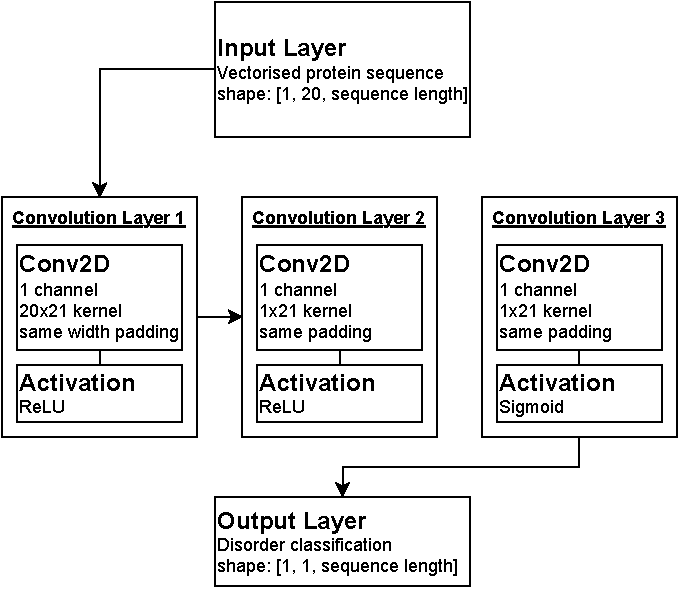
\includegraphics[width=0.75\linewidth]{images/2DCNNdraw.pdf}    

    \caption{A schematic representation of the first CNN. This neural network applies three convolutions to our vectorised protein sequence. These layers use two-dimensional convolution kernels. The first two layers use the ReLU activation function. Our final feature map is given to a sigmoid activation function to return disorder predictions.}

    \label{fig:2DCNN} 
\end{figure}

Our other CNN uses multiple 1D convolution kernels and its network architecture is described in Figure \ref{fig:1DCNN}. We used a convolution kernel of size 21, like the width of our 2D convolution kernels. We found using 10 channels as our hidden dimension helped the model to learn and keeping this channel size as 1, like our 2D CNN, did not work. This model uses the same activation functions as our above model and the BCEWithLogitsLoss loss function. Finally, for this model, we employed dropout because it was overfitting and this regularisation that was added during training helped reduce the overfitting.

\begin{figure}
    \centering
    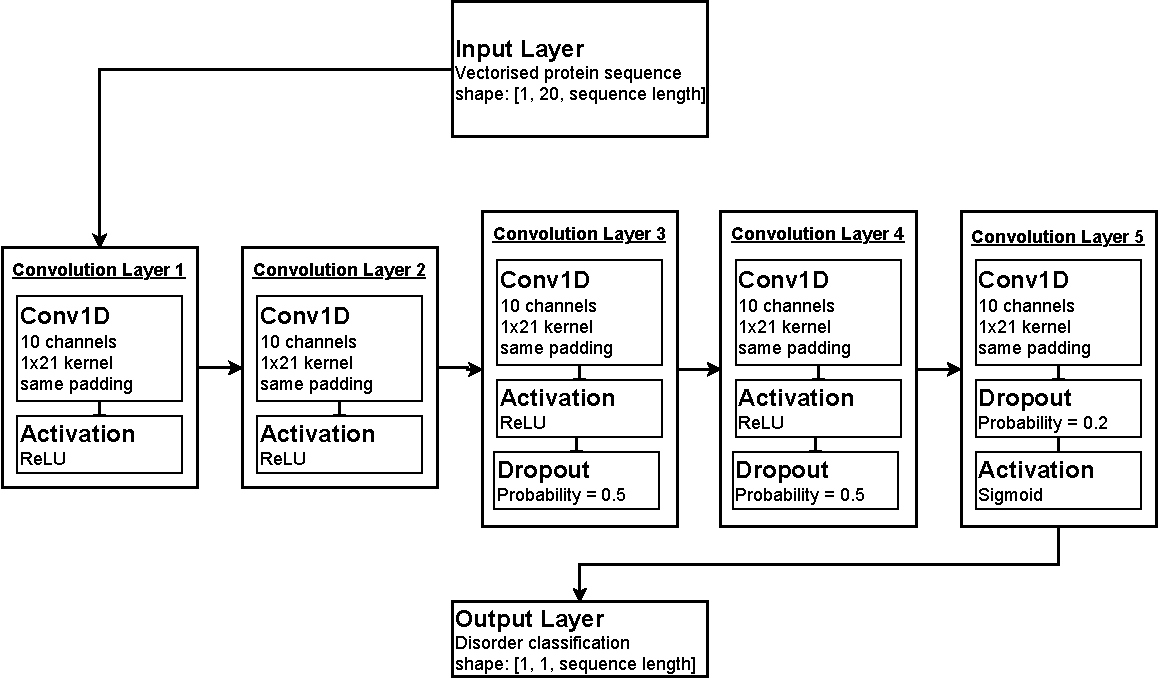
\includegraphics[width=0.95\linewidth]{images/1DCNNdraw.pdf}    

    \caption{A schematic representation of the second CNN. This neural network applies five convolutions to our vectorised protein sequence. These layers use one-dimensional convolution kernels. Network layers use the ReLU activation function, until the final layer where sigmoid is applied. Dropout is used at the end of the network to add regularisation to more complex feature maps.}

    \label{fig:1DCNN} 
\end{figure}


\subsection{RNN}

Our long short-term memory recurrent neural network (LSTM) is bidirectional, and its network architecture is described in Figure \ref{fig:RNN}. We have set batch first as true, meaning that the input shape to our LSTM layer would be [batch size, sequence length, input features]. Our data loader used by the other models returns our sequences as [batch size, input features, sequence length], therefore this input is transposed to fit the required input shape. We did this using PyTorch’s einsum functionality. The hidden states are important in the LSTM, and these are initialised to zero as this is the common approach when initialising the LSTM hidden states. From PyTorch documentation on LSTMs, using all zeros is also the default if no hidden state is created \citep{pytorch}. Furthermore, the hidden state is initialised every new forward pass, therefore it is re-initialised every sequence. This means our hidden state is used to capture dependencies of each sequence separately. Finally, our LSTM is bidirectional, therefore it processes the sequence in both directions: from the beginning to the end and from the end to the beginning, as discussed in our design of RNNs (Section \ref{chap:design section:rnn}).

\begin{figure}[!ht]
    \centering
    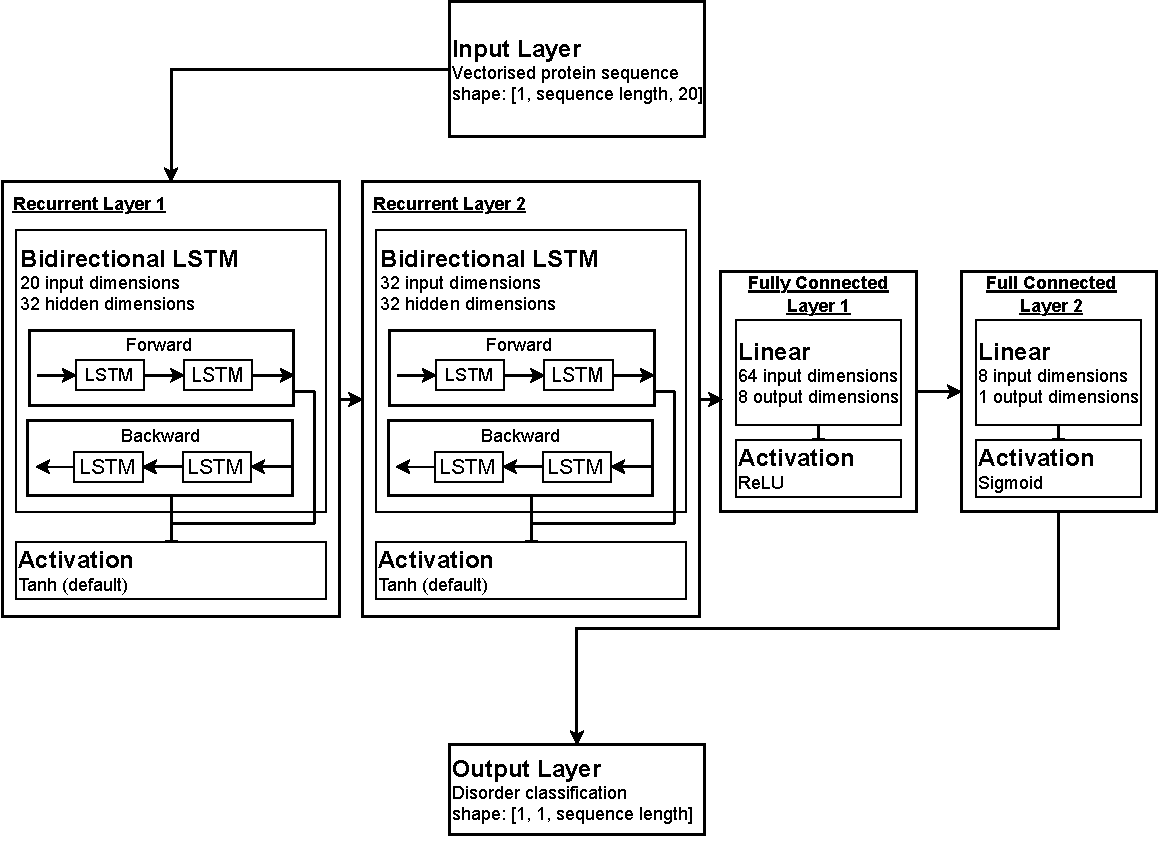
\includegraphics[width=0.95\linewidth]{images/RNNdraw.pdf}    

    \caption{A schematic representation of the LSTM. This neural network applies two stacked bidirectional LSTM layers followed by two fully connected layers to our vectorised protein sequence. These LSTM layers use 32 hidden dimensions, meaning that the LSTM maintains 32 hidden states at once. As our LSTM is bidirectional, it will maintain 64 states at once, hence the first fully connected layer takes in 64 input dimensions. Our final feature map is again given to a sigmoid activation function to return disorder predictions.}

    \label{fig:RNN} 
\end{figure}

\section{Training the network}

All of the models were trained using a training loop, which was run for many epochs. Throughout training, calculations are made more efficient using the CUDA GPU \citep{Nickolls:08}, which can be run on Google Colaboratory. This lowered training times. To utilise CUDA within the training loop we first moved our tensors to this GPU device. Then, our PyTorch training loop is as expected: first evaluating the models' predictions through our BCEWithLogitsLoss loss function, setting our current gradient to zero, using backpropagation through time to calculate a gradient, then making a step with our optimiser from the gradient calculation. Furthermore, as we were using a batch size of one, we experimented with gradient accumulation, which imitates having a larger batch size \citep{Bhattacharyya:20}. This feature did not give improvements to our learning task, so we removed it. The optimiser we used for training was SGD and this was seen to work well with a standard momentum of 0.9, low learning rates and low weight decay values as discussed in our hyperparameter tuning section (Section \ref{chap:implementation section:hyperparameters}).

\section{Hyperparameter optimisation}
\label{chap:implementation section:hyperparameters}
Many options for the depth of these neural networks, the size of neural network layer parameters and optimisers were experimented on. We used the validation dataset to find trained models with a good fit to unseen data. From early manual inspection, we found that most models responded well to low learning rates and low weight decay. We optimised the hyperparameters for all of our final architectures and these final architectures are discussed in Section \ref{chap:implementation sec:architectures}. RayTune \citep{Liaw:18}, a scalable hyperparameter tuning framework, was used to further tune our hyperparameters, given a sensible range of values for the learning rate and regularisation term. We optimised these parameters for the SGD optimiser. Due to computational costs, we only considered 10 parameter combinations for every model. Table \ref{tab:hyperparameters} demonstrates what parameters RayTune selected as they performed best on the validation dataset's loss and were used to train our final models used in our evaluation (Section \ref{chap:evaluation}).

\begin{table}[!ht]
    \centering
    \caption{This table shows the optimal learning rate and weight decay parameters to be used with the SGD optimisation method given different models. Low learning rates and a variety of weight decays were chosen as the optimal parameters.}
    
    \begin{tabular}{|c|ccc|}
    \hline
    Model & \multicolumn{1}{c|}{Feature input} & \multicolumn{1}{c|}{Learning rate} & \multicolumn{1}{c|}{Weight decay (regularisation)} \\ \hline
    \multirow{2}{*}{CNN (2D)} & One-hot & 0.0005 & 0.01 \\ \cline{2-4} 
     & PSSM & 0.0005 & 0.005 \\ \hline
    \multirow{2}{*}{CNN (1D)} & One-hot & 0.0005 & 0.001 \\ \cline{2-4} 
     & PSSM & 0.001 & 0.005 \\ \hline
    \multirow{2}{*}{RNN (LSTM)} & One-hot & 0.001 & 0.001 \\ \cline{2-4} 
     & PSSM & 0.001 & 0.0025 \\ \hline
    \end{tabular}

    \label{tab:hyperparameters} 
\end{table}


\section{Django server}
We have also implemented a small web application to make our solution accessible. This web server has two web pages. These visually follow the wireframes, and this user interface aims to be user-friendly. For our first page, we use a Django form which when submitted sends a POST request where the Django views conducts the classification of the disordered regions in the protein sequence. This form validates that the inputted sequence is a FASTA file and that every amino acid code is one of the 20 recognised amino acids. If these constraints are not satisfied, the classification will not continue as our solution cannot handle invalid amino acids. As we used Python throughout our deep learning evaluation, we have used code from our notebooks in a helper file to generate our features and make a prediction using our best performing model.

Our other page is the sequence visualisation indicating the IDRs using colour: where red implies disorder and green implies order. The purpose of these colours is described as well to improve usability. We implemented the visualisation using a JavaScript function that creates a fake table so that the sequence characters are equally spaced, making the visualisation is pleasant. Furthermore, this table has 60 columns, therefore 60 characters long, because this is how many amino acid characters there are before the newline character in a FASTA file. This was done to maintain consistency with how protein sequences are read.

\subsection{Containerising the web application}

We containerised this web application by setting up a simple Docker, Nginx and Gunicorn configuration. Using this container provides a consistent environment for the application to run, which can help to avoid compatibility issues and is important for ensuring we have access to a suitable version of packages that work with PyTorch for example. Using containers means that a future external database could have a separate container, which promotes security and scalability. Using Nginx and Gunicorn will help a deployed web application handle multiple requests. Overall, this set-up can be used and further maintained to change scalability, performance and security of the web server.




%==================================================================================================================================
\chapter{Evaluation}
\label{chap:evaluation}

\section{Evaluation goal}

Our goal is to evaluate how well different deep neural network architectures and approaches used in deep learning perform against each other when predicting where IDRs are within protein sequences. We have trained six final models. The models are built using three different types of architectures: CNN (2D), CNN (1D), and RNN (LSTM) (Section \ref{chap:implementation sec:architectures}). Each architecture is trained using two types of feature inputs: one-hot encoding and position-specific scoring matrix (PSSM) (Section \ref{chap:implementation sec:features}). We now discuss these model’s performance at protein disorder prediction with questions considering the \textit{“effect of architecture on performance”}, the \textit{“effect of input features on performance”} and how this overall has an effect to the classification of disorder.

\section{How we will assess our deep neural networks}

We will use metrics from Section \ref{chap:design sec:eval}, as these are often used in deep learning. The MCC is especially useful to ensure all our classes have been accurately classified as we have an imbalanced dataset. This MCC will prevent a model that predicts the majority class (ordered amino acids) from being more accurate due to simply predicting the most popular class and not learning meaningful features.

With the metrics, we evaluate the overall performance of each model given unseen protein sequences. As we are assessing multiple sequences, each of which has multiple labels, we will first calculate the micro-average of these metrics for each sequence, meaning that we count the total number of true positives, true negatives, false positives and false negatives for the predictions made for a single sequence and calculate our metrics. We then take an average of these calculated metric scores over all the sequences to report our final scores. This was done because this evaluation should be thought of as the model's performance given a new sequence, therefore it is appropriate to take the average score over these sequences. Furthermore, this approach is used in the literature as protein sequences length and disorder content can vary greatly, meaning it would be difficult to compare metrics directly across different sequences. For example, the metrics could be skewed from an extremely large sequence that is predicted well.

It can be noted that we did calculate these metrics using the sum of the true positives, true negatives, false positives and false negatives over all of the sequences, instead of calculating it for each sequence, but similar conclusions were made about what architectures and approaches performed better. However, calculating metrics in this fashion was valuable as with the total true positive, true negative, false positive and false negative values we constructed confusion matrices to see how often models predicted ordered or disordered labels correctly.

Finally, we will evaluate our model performance using the probability-based classifications discussed in our design (Section \ref{chap:design sec:evalThresh}). With our probability values, we can plot receiver operating characteristic (ROC) curves and calculate the area under the ROC Curve (AUC). This was done so we can evaluate how different thresholds will perform at classifying disorder and how this will affect the true positive rate (TPR) and false positive rate (FPR). This gives us further understanding about our models’ performances.

\section{Classification of DisProt data}
\label{chap:eval sec:test}

\begin{table}[!ht]
    \centering
    \caption{This table shows different models and their performance predicting protein disorder using different evaluation metrics. It is clear PSSM feature input produces better predictions than one-hot encoding. Furthermore, the model architectures of CNN (1D) and the LSTM are competitive against each other, whereas CNN (2D) does not perform as well with this test dataset.}
    \begin{tabular}{|c|c|c|c|c|c|c|c|}
    \hline
    Model architecture & Feature input & Accuracy & Precision & Recall & Specificity & F1-score & MCC \\ \hline
    \multirow{2}{*}{CNN (2D)} & One-hot & 0.4277 & 0.2737 & \textbf{0.9281} & 0.2493 & 0.3603 & 0.1380 \\ \cline{2-8} 
     & PSSM & 0.4953 & 0.2814 & 0.8360 & 0.3595 & 0.3582 & 0.1433 \\ \hline
    \multirow{2}{*}{CNN (1D)} & One-hot & 0.6831 & 0.3541 & 0.6109 & 0.6369 & 0.3748 & 0.2061 \\ \cline{2-8} 
     & PSSM & \textbf{0.6939} & 0.3669 & 0.6514 & \textbf{0.6436} & 0.3980 & 0.2422 \\ \hline
    \multirow{2}{*}{RNN (LSTM)} & One-hot & 0.6258 & 0.3328 & 0.7648 & 0.4977 & 0.4033 & 0.2041 \\ \cline{2-8} 
     & PSSM & 0.6934 & \textbf{0.3734} & 0.6759 & 0.6285 & \textbf{0.4101} & \textbf{0.2490} \\ \hline
    \end{tabular}
    
    \label{tab:testDataset}
\end{table}

The withheld testing dataset we created from DisProt \citep{disprot} was used to evaluate our different model performances first. Table \ref{tab:testDataset} presents the evaluation metrics of these different models with this test set. From the table, we can see that the performance of the models does vary depending on the architecture and feature input used. Between the CNN models, the CNN using 1D convolutions within its architecture outperforms the 2D architecture for both types of feature inputs. The LSTM architecture also performs competitively given our models; giving similar results to the better CNN (1D).

In terms of feature input, we observe that PSSMs outperform one-hot encoding for every model. This suggests that the PSSM feature input may be more informative at expressing features about disordered regions within protein sequences.

Overall, the highest performing models are the CNN (1D) and LSTM architectures with PSSM feature input. This CNN has an accuracy of 0.6939, the highest accuracy for this test dataset and an MCC of 0.2422. This LSTM has an accuracy of 0.6934 and an MCC of 0.2490 which is the highest MCC score on this test dataset. Given that the LSTM architecture also has the highest F1-score (0.4101), we conclude that on this test dataset the LSTM architecture has the best performance.

\subsection{Model confusion}
\label{chap:eval sec:testconfusion}

We can look at each model with more granularity by evaluating the classification report of each model, given by the scikit-learn library \citep{Pedregosa:11}. This looks at the overall true positives, true negatives, false positives and false negatives rather than regarding them for each sequence but is useful to see how well our two different classes, order and disorder, were classified. This gives us information about the overall precision, recall and F1-score of each class and we can also use a confusion matrix to see how much order and disorder was misclassified by different models. \\
\subsubsection{CNNs \newline}
For our CNNs using the 2D convolutions within its architecture, our confusion matrices (Figure \ref{fig:cf2d1hot} and Figure \ref{fig:cf2dpssm}) show that this model is often classifying many ordered residues as disordered. Using the PSSM features lowers this misclassification, but there is still mostly disordered amino acids being predicted, despite the dataset containing a majority of ordered amino acids. This classification distribution helps us understand why the recall for this model is so high (Table \ref{tab:testDataset}), as it is much less likely to misclassify a disordered amino acid because it attempts to classify more amino acids as disordered.

For our CNNs using the 1D convolutions within its architecture, our confusion matrices (Figure \ref{fig:cf1d1hot} and Figure \ref{fig:cf1dpssm}) show there are better classifications being made than the previous CNN architecture. We can see a better balance between the two classes, with a lot more ordered amino acids being classified correctly than incorrectly. We can also see a slight improvement to the predictions made when we use the PSSMs as our feature input. This agrees with our analysis of the test set (Section \ref{chap:eval sec:test}), demonstrating using PSSM features improves the CNN models predictions. From analysing all the confusion matrices, we see that this CNN architecture has the lowest false negatives, which can also be seen in Table \ref{tab:testDataset}, as this model architecture has the greatest specificity.

\begin{figure}[!htb] 
    \centering
    \begin{subfigure}[b]{0.48\textwidth}
        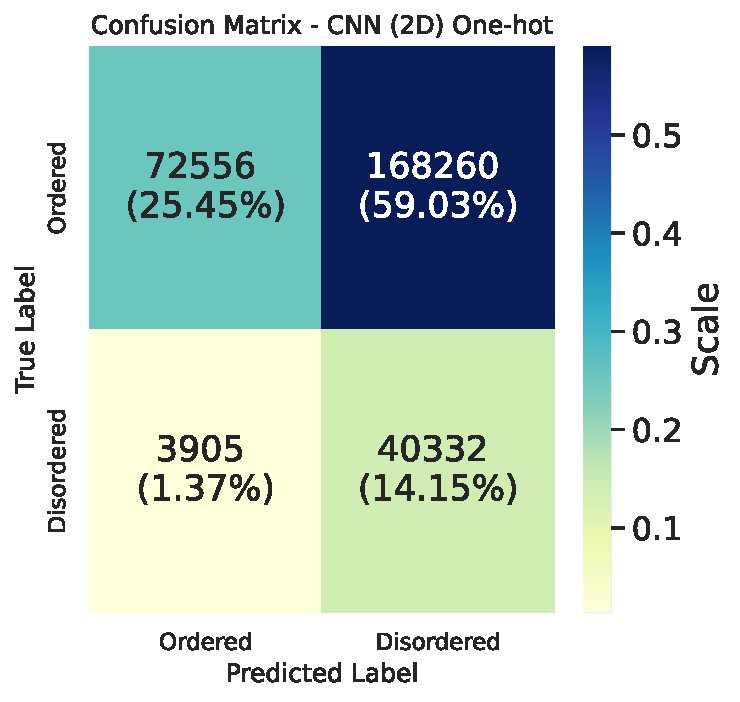
\includegraphics[width=\textwidth]{images/confmats/CNN2D1hot-cf.pdf}
        \caption{One-hot encoding confusion matrix.}
        \label{fig:cf2d1hot}
    \end{subfigure}
    ~
    \begin{subfigure}[b]{0.48\textwidth}
        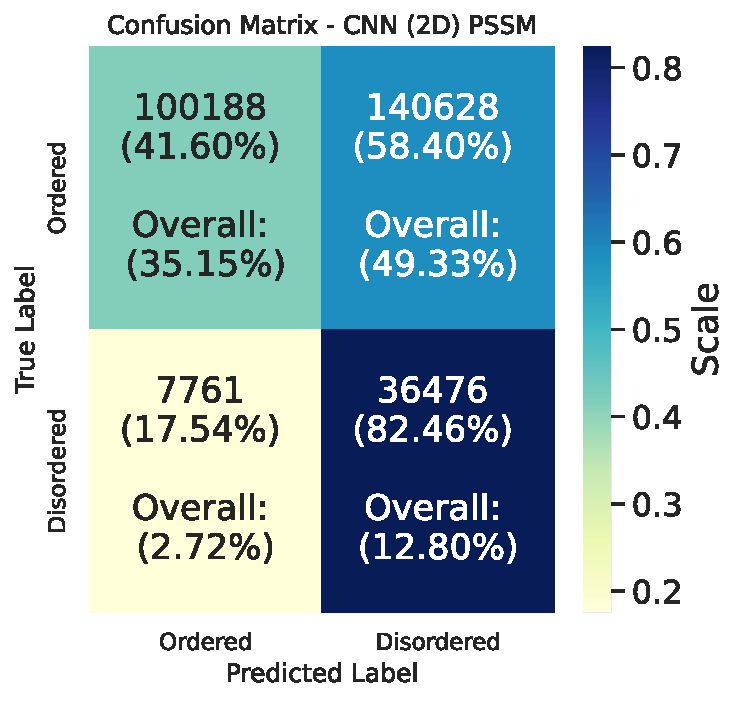
\includegraphics[width=\textwidth]{images/confmats/CNN2Dpssm-cf.pdf}
        \caption{PSSM confusion matrix.}
        \label{fig:cf2dpssm}
    \end{subfigure}
    \caption{Confusion matrices for CNN with 2D convolution kernels within its architecture. \subref{fig:cf2d1hot} shows the confusion matrix for the model using one-hot encoding feature input. \subref{fig:cf2dpssm} shows the confusion matrix for the model using one-hot encoding feature input. We see this models architecture...}
    \label{fig:cf2d}
\end{figure}

\begin{figure}[!htb] 
    \centering
    \begin{subfigure}[b]{0.48\textwidth}
        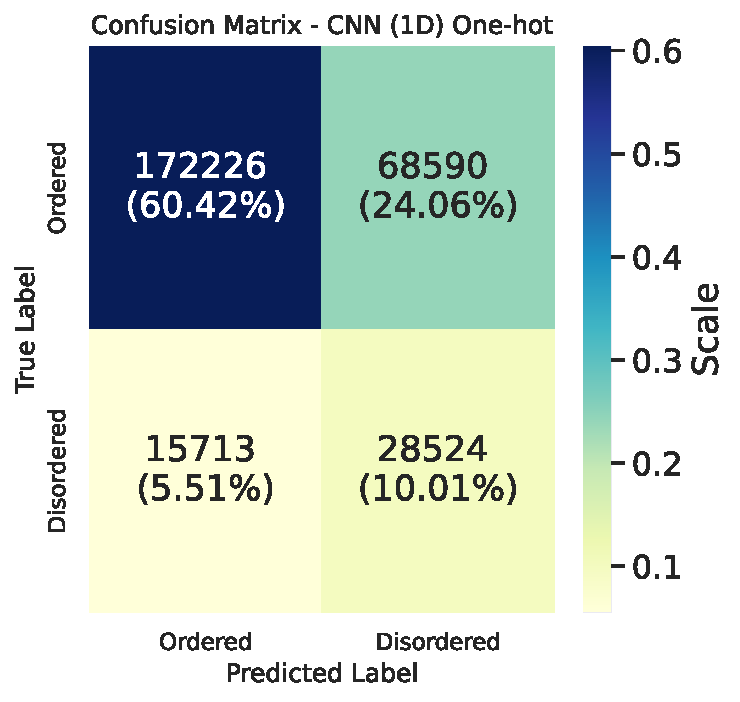
\includegraphics[width=\textwidth]{images/confmats/CNN1D1hot-cf.pdf}
        \caption{One-hot encoding confusion matrix.}
        \label{fig:cf1d1hot}
    \end{subfigure}
    ~
    \begin{subfigure}[b]{0.48\textwidth}
        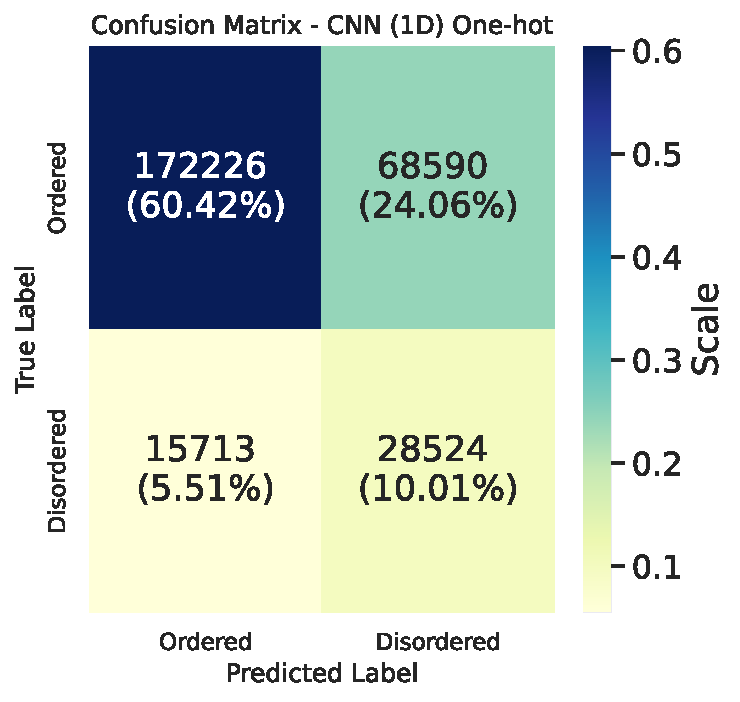
\includegraphics[width=\textwidth]{images/confmats/CNN1D1hot-cf.pdf}
        \caption{PSSM confusion matrix.}
        \label{fig:cf1dpssm}
    \end{subfigure}
    \caption{Confusion matrices for CNN with 1D convolution kernels within its architecture. \subref{fig:cf2d1hot} shows the confusion matrix for the model using one-hot encoding feature input. \subref{fig:cf2dpssm} shows the confusion matrix for the model using one-hot encoding feature input. We see this models architecture...}
    \label{fig:cf1d}
\end{figure}

\subsubsection{RNNs \newline}
Finally, our RNNs, using a LSTM architecture, can be regarded as the best model architecture for predicting IDRs in the protein sequences of our test dataset. Our confusion matrices (Figure \ref{fig:cfrnn1hot} and Figure \ref{fig:cfrnnpssm}) help demonstrate how many ordered and disordered amino acids were misclassified by models using the LSTM architecture. Considering the different feature inputs, our one-hot encoding method tends to classify more disordered amino acids correctly at the cost of misclassifying more ordered amino acids as disordered. Whereas, the PSSM inputs have less misclassified ordered amino acids, but the model has a weaker recall and has predicted less disordered amino acids correctly.

\begin{figure}[!htb] 
    \centering
    \begin{subfigure}[b]{0.48\textwidth}
        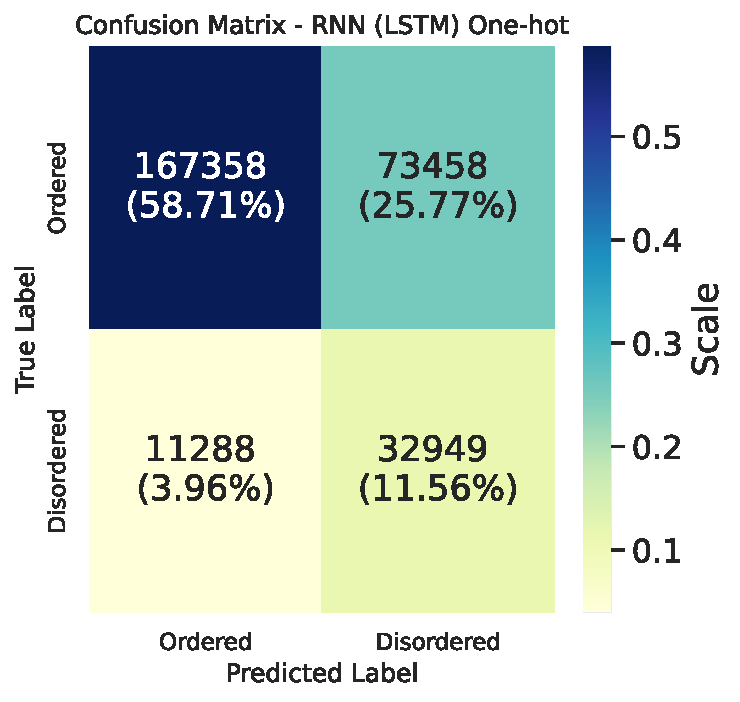
\includegraphics[width=\textwidth]{images/confmats/RNN1hot-cf.pdf}
        \caption{One-hot encoding confusion matrix.}
        \label{fig:cfrnn1hot}
    \end{subfigure}
    ~
    \begin{subfigure}[b]{0.48\textwidth}
        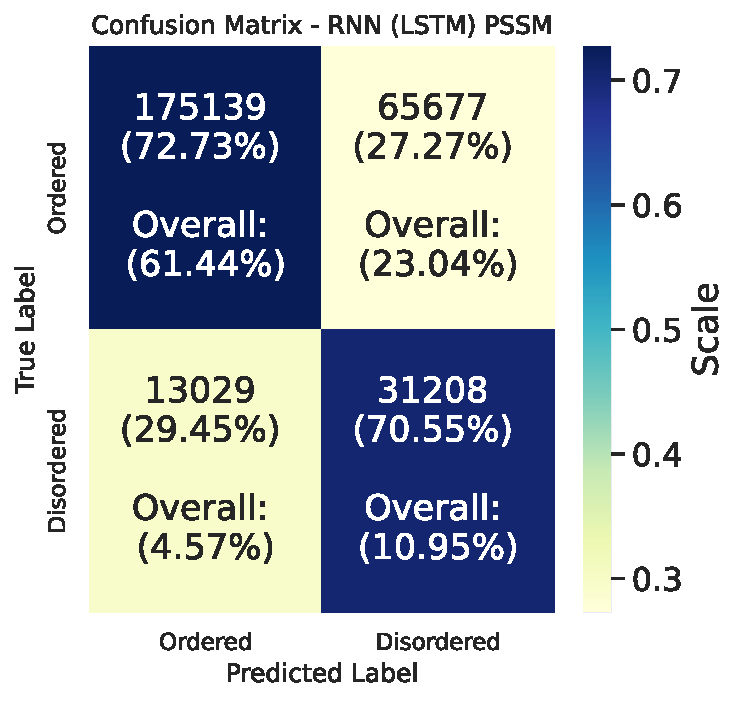
\includegraphics[width=\textwidth]{images/confmats/RNNpssm-cf.pdf}
        \caption{PSSM confusion matrix.}
        \label{fig:cfrnnpssm}
    \end{subfigure}
    \caption{Confusion matrices for CNN with 2D convolution kernels within its architecture. \subref{fig:cf2d1hot} shows the confusion matrix for the model using one-hot encoding feature input. \subref{fig:cf2dpssm} shows the confusion matrix for the model using one-hot encoding feature input. We see this models architecture...}
    \label{fig:cfrnn}
\end{figure}

\subsection{Analysis of probability-based predictions}

\begin{figure}[!htb]
    \centering
    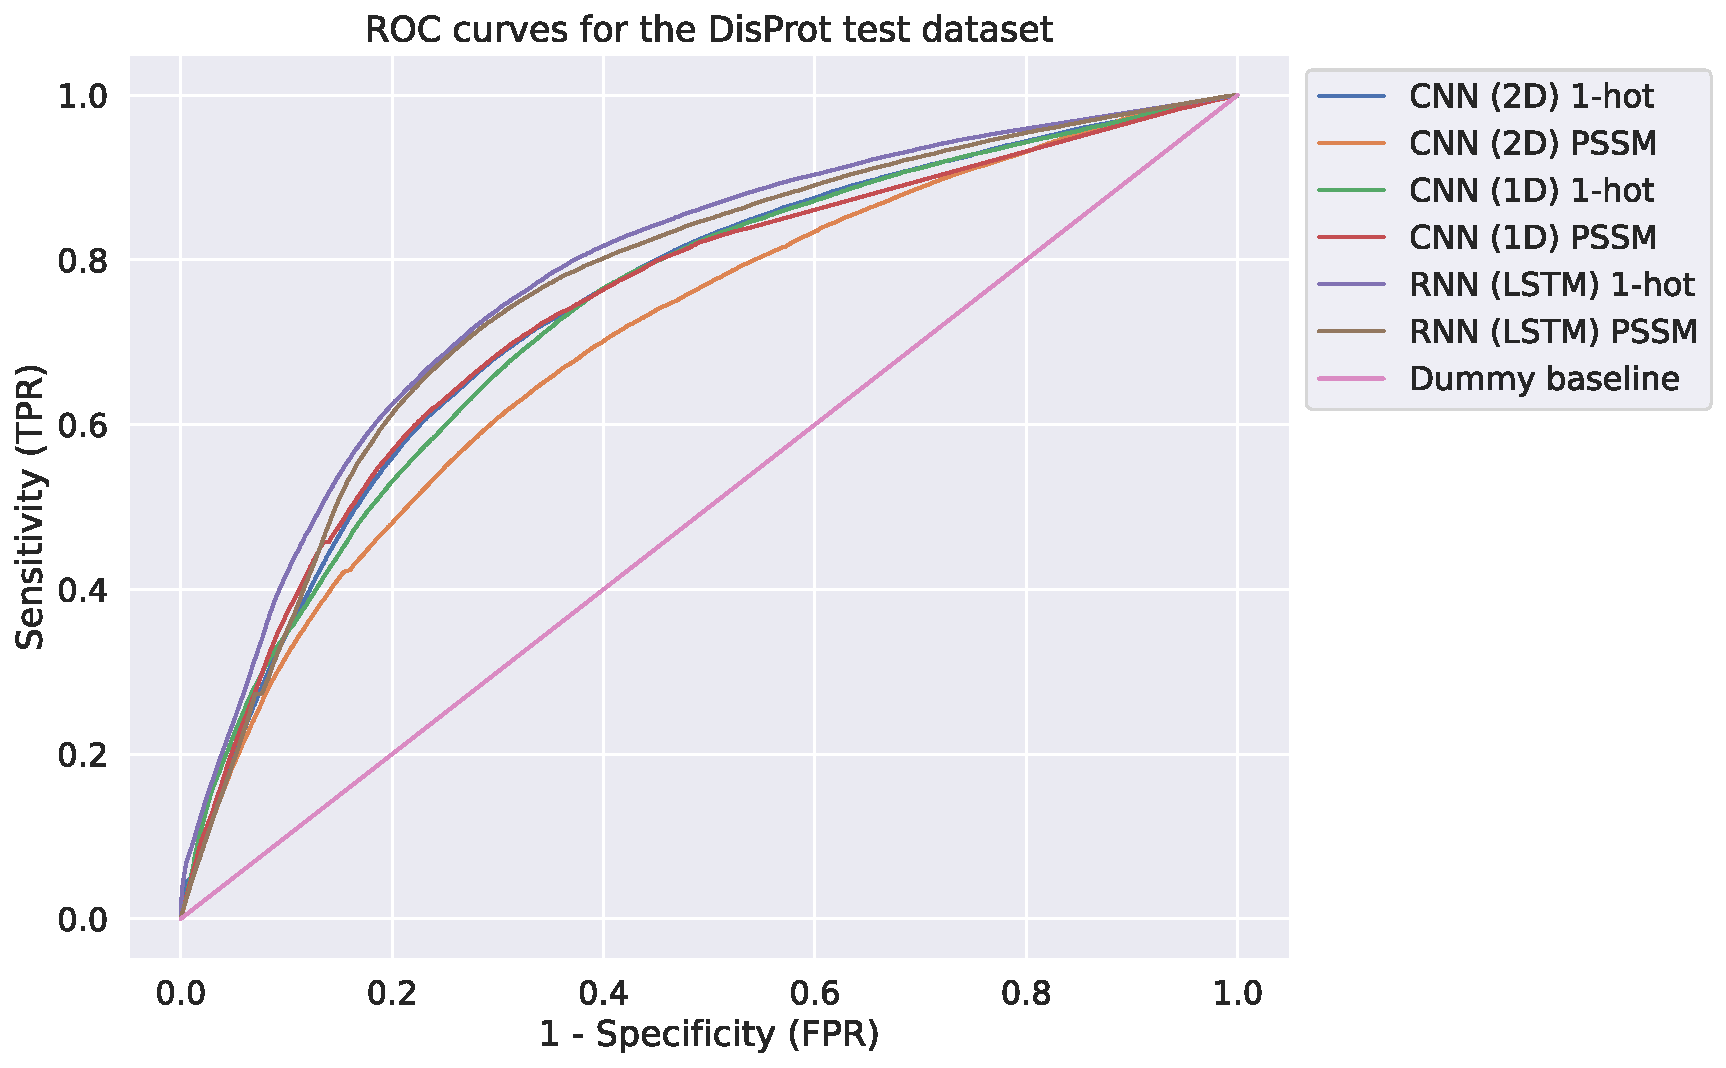
\includegraphics[width=0.95\linewidth]{images/DisProtROC.pdf}    

    \caption{ROC curves of probability-based IDR predictions for our 6 models on the withheld DisProt test data.}

    \label{fig:roctest} 
\end{figure}

With our DisProt test dataset Figure \ref{fig:roctest} demonstrates that our LSTM with PSSM feature input is the best model in terms of trade-off between the true positive rate (TPR) and false positive rate (FPR). This agrees with our evaluation using our other metrics such as MCC and F1-score. The two models using the LSTM architecture have a higher area under the ROC Curve (AUC), showing the LSTM is better at identifying IDRs within protein sequences. The CNN models have a slightly lower performance than the LSTMs when using this metric; with the 2D CNN with PSSM input having the worst performance at correctly classifying confidently. However, all of these classifiers perform better than a dummy baseline. This can be seen in Figure \ref{fig:roctest} because, at 0.5 true positives there are less than 0.5 false positives; with the worst classifier only recording 0.2 false positives at 0.5 true positives.

\section{Classification of CASP10 data}
\label{chap:eval sec:casp10}

\begin{table}[!ht]
    \centering
    \caption{This table shows different models and their performance predicting protein disorder using different evaluation metrics on the CASP10 dataset.}
    \begin{tabular}{|c|c|c|c|c|c|c|c|}
    \hline
    Model architecture & Feature input & Accuracy & Precision & Recall & Specificity & F1-score & MCC \\ \hline
    \multirow{2}{*}{CNN (2D)} & One-hot & 0.6351 & 0.1766 & 0.5551 & 0.6466 & 0.2256 & 0.1195 \\ \cline{2-8} 
     & PSSM & 0.4461 & 0.156 & 0.7758 & 0.3967 & 0.2318 & 0.0982 \\ \hline
    \multirow{2}{*}{CNN (1D)} & One-hot & \textbf{0.7401} & 0.2148 & 0.4367 & \textbf{0.7647} & 0.2458 & 0.1587 \\ \cline{2-8} 
     & PSSM & 0.7045 & 0.2279 & 0.5819 & 0.7096 & 0.2895 & \textbf{0.1909} \\ \hline
    \multirow{2}{*}{RNN (LSTM)} & One-hot & 0.5414 & 0.1959 & \textbf{0.7891} & 0.4869 & 0.2775 & 0.1636 \\ \cline{2-8} 
     & PSSM & 0.6596 & \textbf{0.2337} & 0.6108 & 0.6479 & \textbf{0.2896} & 0.1809 \\ \hline
    \end{tabular}
    
    \label{tab:caspDataset}
\end{table}

The CASP10 dataset has been used to assess many protein disorder prediction tools. There are 94 targets (protein sequences) in this dataset that were used for analysis as some other sequences proposed in this dataset were removed by the organisers before or during the competition \citep{Moult:14}. For this dataset, we generate one-hot encoded and PSSM features similarly to our DisProt dataset. Furthermore, no sequences in this dataset were invalid for our vectorisation process and model input; therefore, no sequences had to be removed.

We performed a similar analysis on the CASP dataset as we have done using the DisProt withheld test dataset. We used the same model architectures and features as above but trained out models using our entire DisProt dataset before making predictions on the CASP dataset. Table \ref{tab:caspDataset} presents the evaluation metrics of our different models' performances on the CASP10 dataset. From this table, we see a similar performance difference between the architectures and feature inputs as the previous unseen test dataset. Again, the CNN using 2D convolutions within its architecture has the worst performance. For the CNN using 1D convolutions and the LSTM it is clear again that using the PSSMs as our feature input does improve the prediction quality of protein disorder. Both of these models are once again comparably competitive, with the CNN model achieving the highest MCC of 0.1909 and the LSTM has the highest F1-score of 0.2896. It is also interesting to note that the with better CNN architecture, a model using one-hot encoding has the highest accuracy and specificity measure. Overall, we claim the CNN (1D) using PSSM features has the leading performance as it has the strongest distribution of metrics. However, we can see that both the CNN (1D) and LSTM perform similarly with the CASP10 dataset, making it more difficult to justify a best architecture. This has demonstrated the capability of different network architectures at this task.

\subsection{Model confusion}

Using our different model architectures and feature inputs predictions on the CASP dataset, we have seen similarities and differences to the confusion shown about predictions on our test dataset (Section \ref{chap:eval sec:testconfusion}).

\subsubsection{CNNs \newline}

For the CNN architecture with 2D convolution kernels, the two models that use different feature inputs have very different confusion matrices. With one-hot encoding features, our model classifies half of the disordered amino acids correctly (Figure \ref{fig:caspcf2d1hot}), whereas the model using PSSM features classifies three-quarters of these disordered amino acids correctly at the expense of classifying more than half of the ordered amino acids incorrectly (Figure \ref{fig:caspcf2dpssm}). This is similar to this architecture’s performance on the DisProt test dataset (Section \ref{chap:eval sec:testconfusion}), where we saw that it often over-predicted disordered amino acids. This means this model has likely been unable to capture the unique intricate features that represent IDRs.

The CNN architecture with 1D convolution kernels classifies only approximately half of the disordered amino acids correctly for both feature inputs, which can be seen by Figure \ref{fig:caspcf1d1hot} and Figure \ref{fig:caspcf1dpssm}. We can see the CNN with one-hot encoding features, which is our most accurate model (Table \ref{tab:caspDataset}), performs worse at classifying disordered amino acids, and the CNN with PSSM features performs worse at classifying ordered amino acids. However, this difference is not significant enough to determine the least confused model.

\begin{figure}[!htb] 
    \centering
    \begin{subfigure}[b]{0.48\textwidth}
        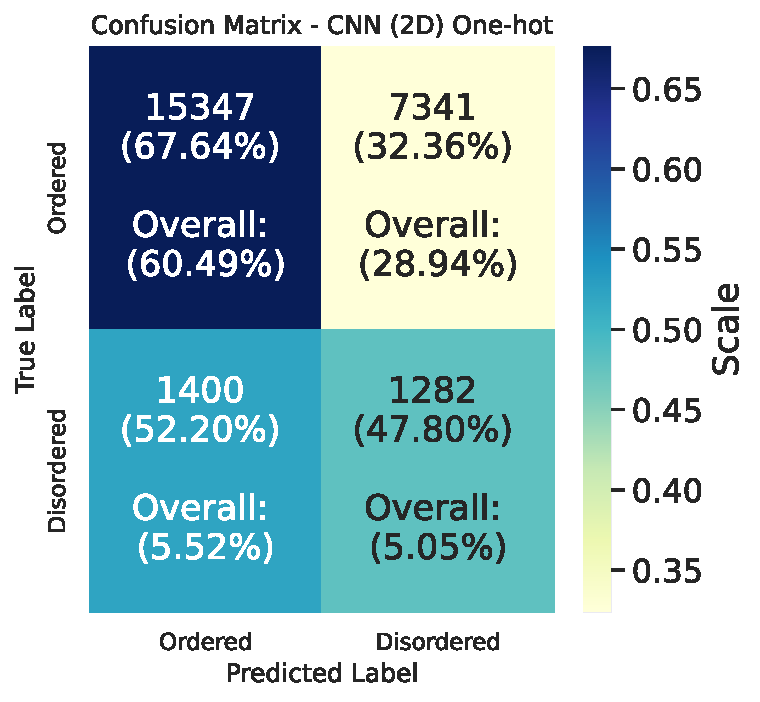
\includegraphics[width=\textwidth]{images/confmats/CASP10CNN2D1hot-cf.pdf}
        \caption{One-hot encoding confusion matrix.}
        \label{fig:caspcf2d1hot}
    \end{subfigure}
    ~
    \begin{subfigure}[b]{0.48\textwidth}
        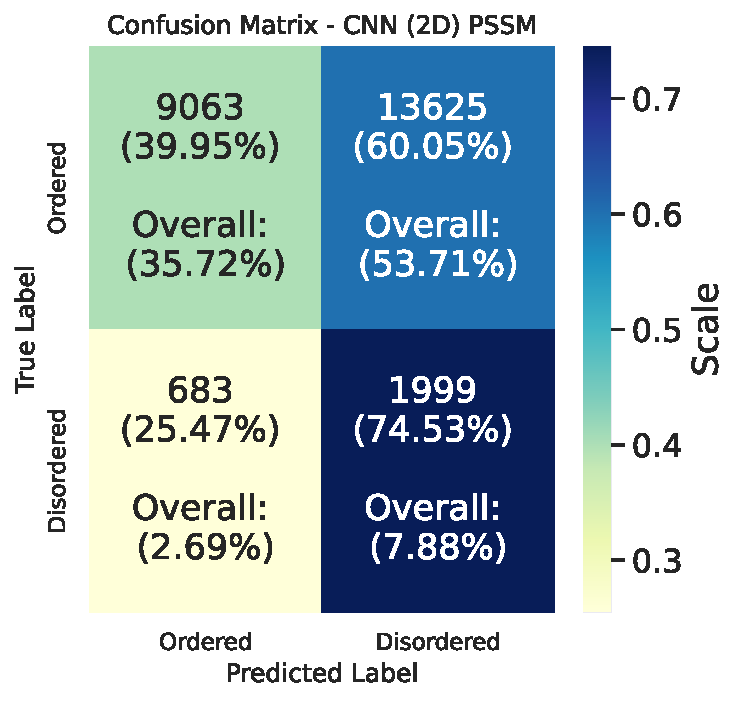
\includegraphics[width=\textwidth]{images/confmats/CASP10CNN2Dpssm-cf.pdf}
        \caption{PSSM confusion matrix.}
        \label{fig:caspcf2dpssm}
    \end{subfigure}
    \caption{Confusion matrices for CNN with 2D convolution kernels within its architecture. \subref{fig:cf2d1hot} shows the confusion matrix for the model using one-hot encoding feature input. \subref{fig:cf2dpssm} shows the confusion matrix for the model using one-hot encoding feature input. We see this models architecture...}
    \label{fig:caspcf2d}
\end{figure}

\begin{figure}[!htb] 
    \centering
    \begin{subfigure}[b]{0.48\textwidth}
        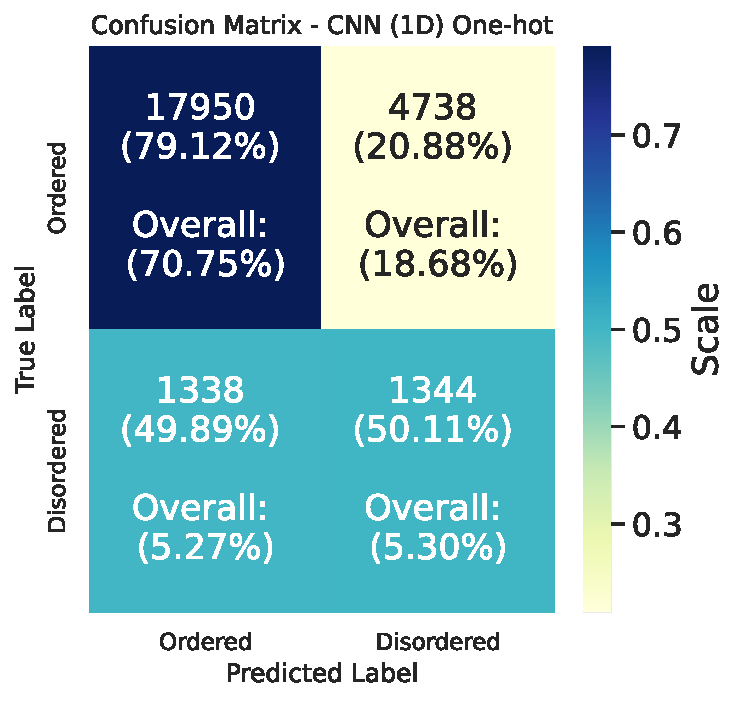
\includegraphics[width=\textwidth]{images/confmats/CASP10CNN1D1hot-cf.pdf}
        \caption{One-hot encoding confusion matrix.}
        \label{fig:caspcf1d1hot}
    \end{subfigure}
    ~
    \begin{subfigure}[b]{0.48\textwidth}
        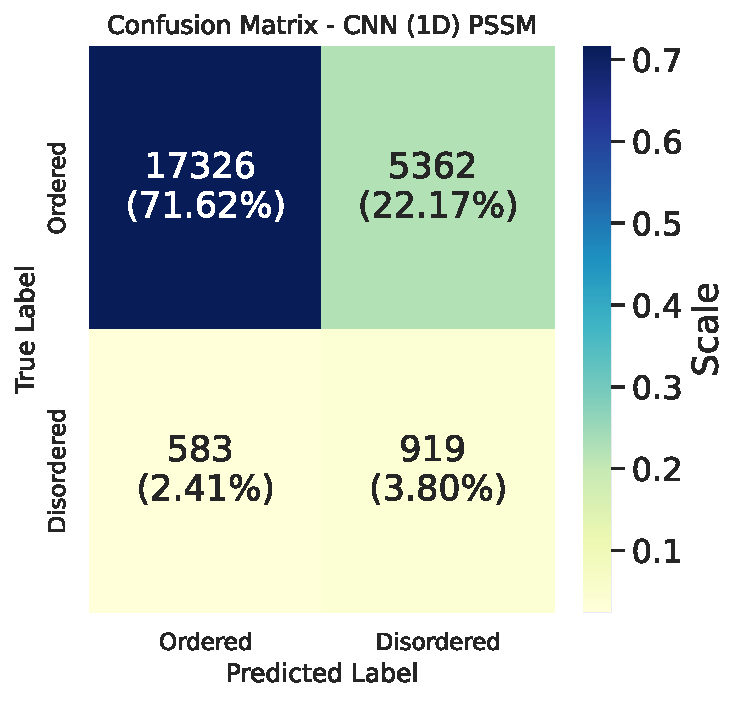
\includegraphics[width=\textwidth]{images/confmats/CASP10CNN1Dpssm-cf.pdf}
        \caption{PSSM confusion matrix.}
        \label{fig:caspcf1dpssm}
    \end{subfigure}
    \caption{Confusion matrices for CNN with 1D convolution kernels within its architecture. \subref{fig:cf2d1hot} shows the confusion matrix for the model using one-hot encoding feature input. \subref{fig:cf2dpssm} shows the confusion matrix for the model using one-hot encoding feature input. We see this models architecture...}
    \label{fig:caspcf1d}
\end{figure}

\subsubsection{RNNs \newline}

Our RNN models have less confusion. For the LSTM when one-hot encoding is used, we can see slight overestimations of disorder again. This model also produces the lowest false negative value (when a disordered label is predicted as ordered). However, despite overestimating disordered labels, this model is often a lot less confused about ordered amino acids (Figure \ref{fig:caspcfrnn1hot}) when we compare this model to our other model that overestimates disorder (the 2D CNN). From our confusion matrix of the LSTM with PSSM features (Figure \ref {fig:caspcfrnnpssm}) we can see that it can correctly predict more than half of the disordered amino acids, which is better than the competitive CNN (1D) model. However, the proportion of correctly predicted disordered amino acids is still lower than our DisProt dataset for this model. Overall, the LSTM does get more confused when classifying ordered amino acids when we compare it to our CNN (1D) models; however, in general we can see the LSTM architecture can correctly predict more disordered amino acids while still reasonably predicting ordered amino acids correctly. This is important in our prediction task, and we assert the LSTM architecture exhibits the lowest level of confusion in the CASP10 dataset task.

\begin{figure}[!htb] 
    \centering
    \begin{subfigure}[b]{0.48\textwidth}
        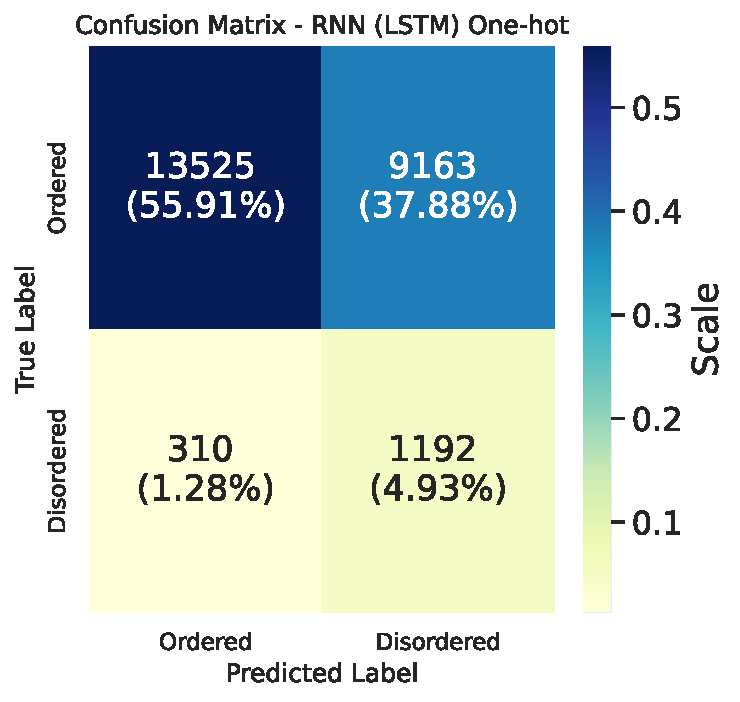
\includegraphics[width=\textwidth]{images/confmats/CASP10RNN1hot-cf.pdf}
        \caption{One-hot encoding confusion matrix.}
        \label{fig:caspcfrnn1hot}
    \end{subfigure}
    ~
    \begin{subfigure}[b]{0.48\textwidth}
        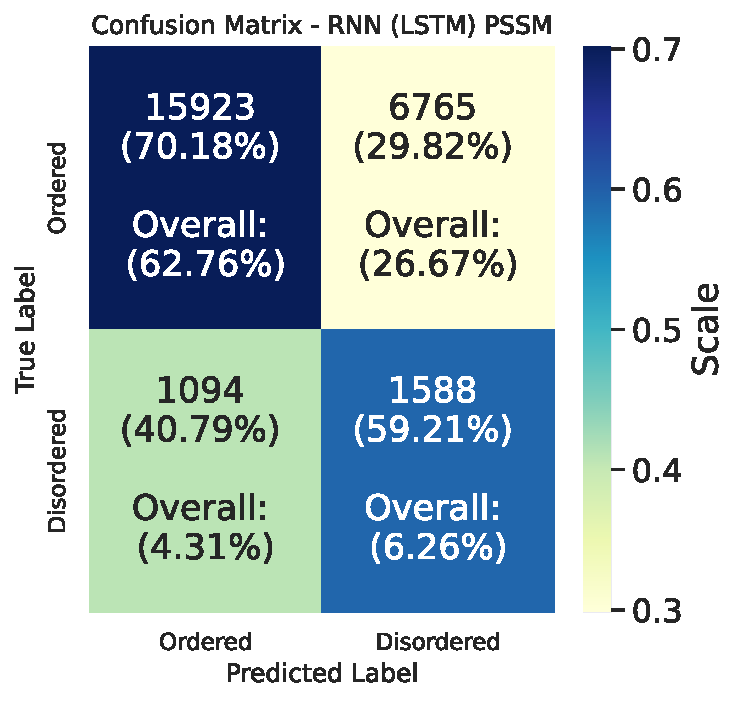
\includegraphics[width=\textwidth]{images/confmats/CASP10RNNpssm-cf.pdf}
        \caption{PSSM confusion matrix.}
        \label{fig:caspcfrnnpssm}
    \end{subfigure}
    \caption{Confusion matrices for CNN with 1D convolution kernels within its architecture. \subref{fig:cf2d1hot} shows the confusion matrix for the model using one-hot encoding feature input. \subref{fig:cf2dpssm} shows the confusion matrix for the model using one-hot encoding feature input. We see this models architecture...}
    \label{fig:caspcfrnn}
\end{figure}

\subsection{Analysis of probability-based predictions}

\begin{figure}[!htb]
    \centering
    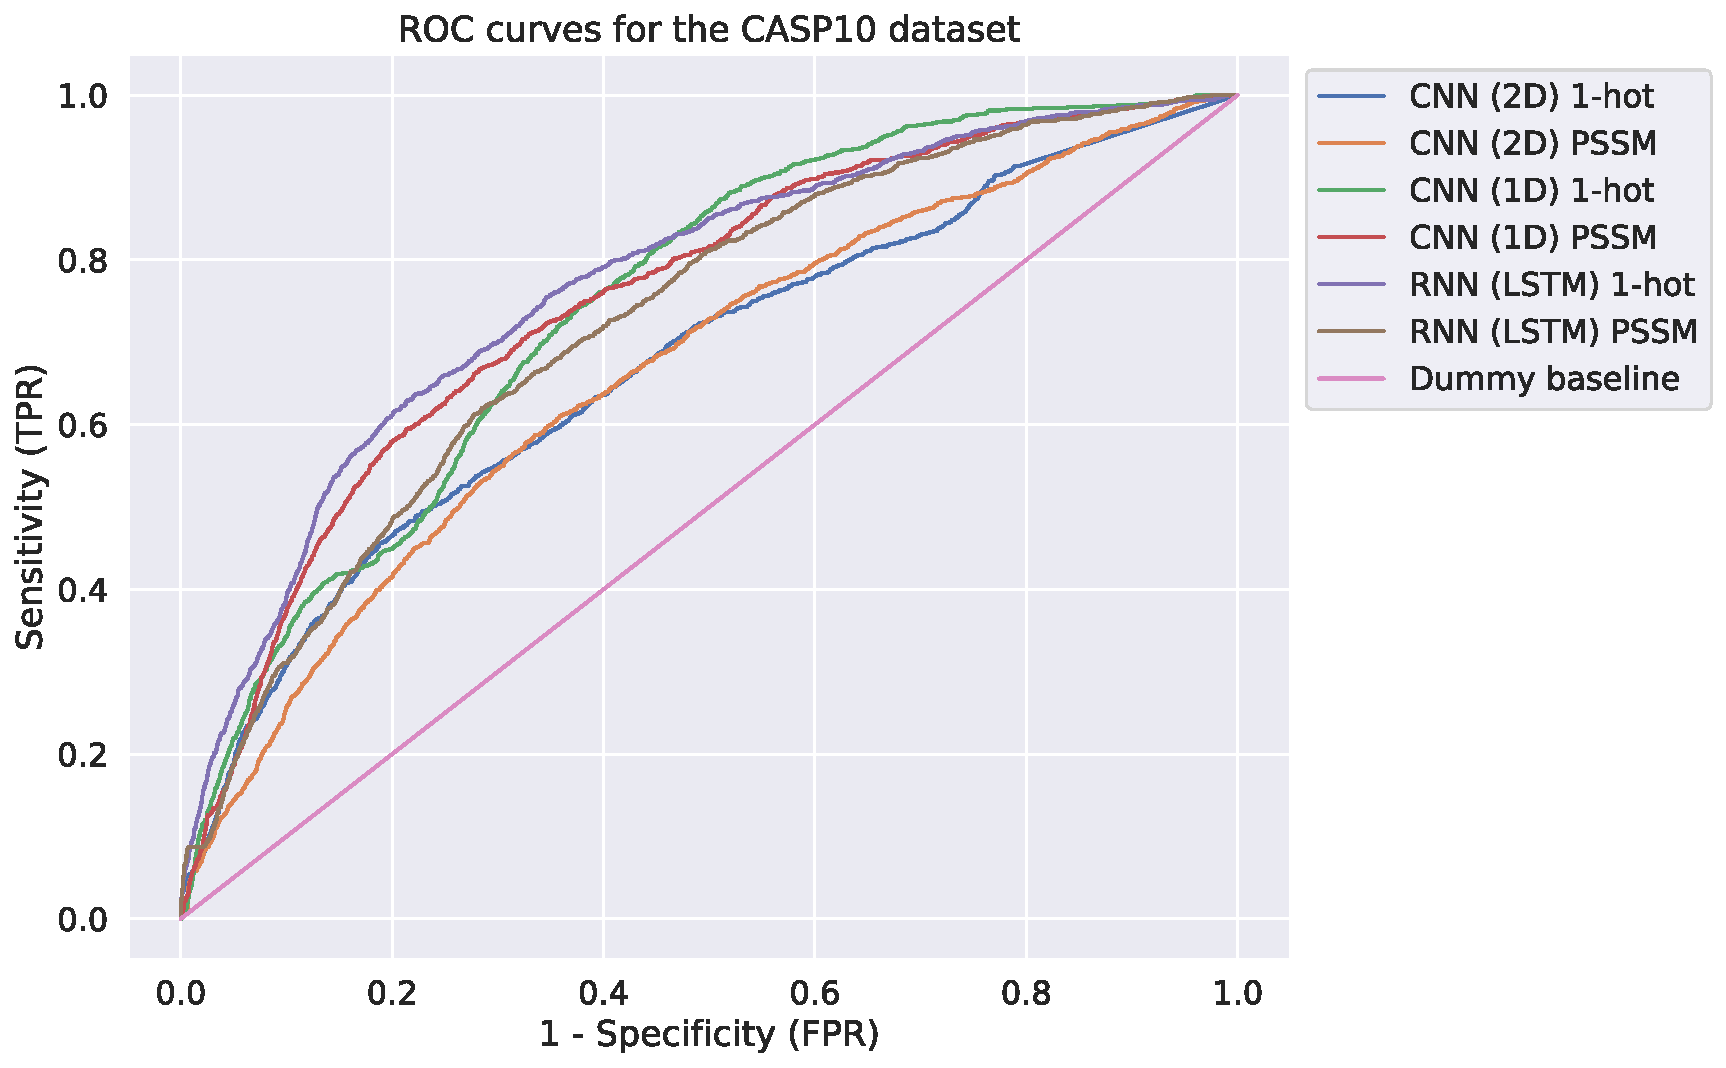
\includegraphics[width=0.95\linewidth]{images/CASPROC.pdf}    

    \caption{ROC curves of probability-based IDR predictions for our 6 models on the withheld DisProt test data.}

    \label{fig:roccasp} 
\end{figure}

When analysing ROC curves with our CASP10 dataset, we see that the CNN (1D) and LSTM using one-hot encoding features achieve the best AUC. This is interesting because it is a different conclusion compared to the other results. We notice when considering the CNN (1D) and LSTM architectures that the one-hot encoding ROC curves are similar and the PSSM ROC curves are similar. This implies that different feature encodings may represent protein sequences in a fashion that different architectures can easily pickup feature patterns. We again conclude that the CNN with 2D convolutions in its architecture has the worst performance on this dataset. Furthermore, we can conclude that all of these models again perform better than the dummy baseline from inspection of that ROC curve graph \ref{fig:roccasp}, demonstrating at 0.5 true positive rate, the false positive rate is below 0.5 for all models.





\newpage

How good is your solution? How well did you solve the general problem, and what evidence do you have to support that?

\section{Guidance}
\begin{itemize}
    \item
        Ask specific questions that address the general problem.
    \item
        Answer them with precise evidence (graphs, numbers, statistical
        analysis, qualitative analysis).
    \item
        Be fair and be scientific.
    \item
        The key thing is to show that you know how to evaluate your work, not
        that your work is the most amazing product ever.
\end{itemize}

\section{Evidence}
Make sure you present your evidence well. Use appropriate visualisations, reporting techniques and statistical analysis, as appropriate.

If you visualise, follow the basic rules, as illustrated in Figure \ref{fig:boxplot}:
\begin{itemize}
\item Label everything correctly (axis, title, units).
\item Caption thoroughly.
\item Reference in text.
\item \textbf{Include appropriate display of uncertainty (e.g. error bars, Box plot)}
\item Minimize clutter.
\end{itemize}

See the file \texttt{guide\_to\_visualising.pdf} for further information and guidance.

\begin{figure}
    \centering
    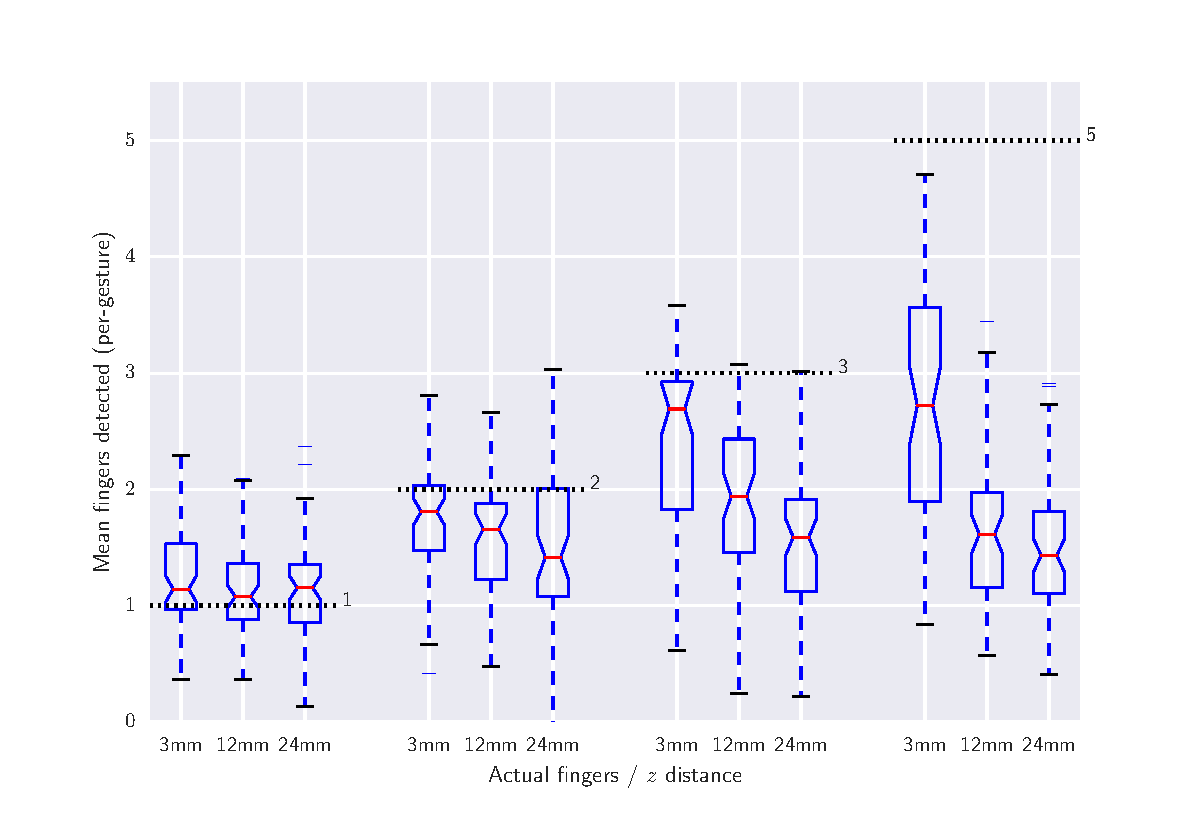
\includegraphics[width=1.0\linewidth]{images/boxplot_finger_distance.pdf}    

    \caption{Average number of fingers detected by the touch sensor at different heights above the surface, averaged over all gestures. Dashed lines indicate
    the true number of fingers present. The Box plots include bootstrapped uncertainty notches for the median. It is clear that the device is biased toward 
    undercounting fingers, particularly at higher $z$ distances.
    }

    % use the notation fig:name to cross reference a figure
    \label{fig:boxplot} 
\end{figure}


%==================================================================================================================================
\chapter{Conclusion}    
Summarise the whole project for a lazy reader who didn't read the rest (e.g. a prize-awarding committee).
\section{Guidance}
\begin{itemize}
    \item
        Summarise briefly and fairly.
    \item
        You should be addressing the general problem you introduced in the
        Introduction.        
    \item
        Include summary of concrete results (``the new compiler ran 2x
        faster'')
    \item
        Indicate what future work could be done, but remember: \textbf{you
        won't get credit for things you haven't done}.
\end{itemize}

%==================================================================================================================================
%
% 
%==================================================================================================================================
%  APPENDICES  

\begin{appendices}

\chapter{Appendices}

Typical inclusions in the appendices are:

\begin{itemize}
\item
  Copies of ethics approvals (required if obtained)
\item
  Copies of questionnaires etc. used to gather data from subjects.
\item
  Extensive tables or figures that are too bulky to fit in the main body of
  the report, particularly ones that are repetitive and summarised in the body.

\item Outline of the source code (e.g. directory structure), or other architecture documentation like class diagrams.

\item User manuals, and any guides to starting/running the software.

\end{itemize}

\textbf{Don't include your source code in the appendices}. It will be
submitted separately.

\end{appendices}

%==================================================================================================================================
%   BIBLIOGRAPHY   

% The bibliography style is abbrvnat
% The bibliography always appears last, after the appendices.

\bibliographystyle{abbrvnat}

\bibliography{l4proj}

\end{document}
